\documentclass [11pt,a4paper]{article}
\usepackage{graphicx,subfigure}
%\documentstyle [epsf,epsfig,11pt,amssymb]{article}
\usepackage{rotating}
\usepackage{lsstdesc_macros}
\usepackage[title]{appendix}

\RequirePackage[colorlinks,breaklinks]{hyperref}  
\hypersetup{linkcolor=blue,citecolor=blue,filecolor=black,urlcolor=blue} 
\usepackage{longtable}
\usepackage{natbib}
\usepackage{verbatim}
%\usepackage{subcaption}

% Set up generic page
%
%\setlength{\textheight}{23cm}
%\setlength{\textwidth}{17cm}
%\unitlength 1mm
%\font\ninerm=cmr9

\textwidth=16.cm
%\textheight=26cm
\setlength{\hoffset}{-1.cm}
\setlength{\voffset}{-1.cm}
\parskip=0.1cm

%\newcommand{\ttt}{{\mbox{\newfont t}}}

\newcommand{\cosmos}{COSMOS}
\newcommand{\xmmlss}{XMM-LSS}
\newcommand{\cdfs}{CDFS}
\newcommand{\elais}{ELAIS-S1}
\newcommand{\spt}{SPT DEEP}
\newcommand{\ddfa}{DDF\_820}
\newcommand{\ddfb}{DDF\_858}
\newcommand{\ddfc}{DDF\_1200}
\newcommand{\ddfd}{DDF\_2689}
\newcommand{\feature}{feature\_baseline\_10yrs}
\newcommand{\strech}{$X_1$}
\newcommand{\sncolor}{$c$}
\newcommand{\daymax}{$T_0$}
\newcommand{\redshift}{$z$}
\newcommand{\tmin}{$T_{min}$}
\newcommand{\tmax}{$T_{max}$}
\newcommand{\phasemin}{$ph_{min}$}
\newcommand{\phasemax}{$ph_{max}$}
\newcommand{\tgapcosmos}{$T_{gap}^{\cosmos}$}
\newcommand{\tgapothers}{$T_{gap}^{others}$}
\newcommand{\zfaint}{$z_{\mathrm{faint}}\ $}
\newcommand{\nsnfaint}{$N_{z<z_{\mathrm{faint}}}\ $}
\newcommand{\zmed}{$z_{\mathrm{med}}\ $}
\newcommand{\nsnmed}{$N_{z<z_{\mathrm{med}}}\ $}
\newcommand{\FixMe}[1]{{\color{red} \bf \large #1}}
\newcommand{\opsim}{{\tt OpSim\ }}
\newcommand{\slair}{{\tt SLAIR\ }}
\newcommand{\altschedsched}{{\tt AltSched\ }}
\newcommand{\altsched}{{\tt altsched\ }}
\newcommand{\myparagraph}[1]{\paragraph{#1}\mbox{}\\}

\graphicspath{{Figures/}}

\begin{document}

\renewcommand\appendix{\par
  \setcounter{section}{0}
  \setcounter{subsection}{0}
  \setcounter{figure}{0}
  \setcounter{table}{0}
  \renewcommand\thesection{Appendix} %\Alph{section}}
  \renewcommand\thefigure{\Alph{section}\arabic{figure}}
  \renewcommand\thetable{\Alph{section}\arabic{table}} 
}

\begin{titlepage}
   \vspace*{\stretch{1.0}}
   \begin{center}
      \Large\textbf{Final assessment for the white paper call}\\
        \vspace*{0.5cm}
      \Large\textbf{DESC-SN group} \\
      
		  \vspace*{0.5cm}

      \large\textit{T. Allam Jr.,R.Biswas, J.Carrick, Ph.Gris, R.Hlo\v{z}ek, I.Hook, A.Kim, M.Lochner, J.McEwen, H. Peiris, N.Regnault, R. Schuhmann, C.Setzer} \\
	\vspace*{0.5cm}

      \large\textit{September 21 2018}
   \end{center}
   \vspace*{\stretch{2.0}}
\end{titlepage}


\tableofcontents


\section{Introduction}



SN cosmology is systematics-limited. Increasing the statistics in the
Hubble diagram must be coupled with (1) advances in the measurement of
the SN distances (i.e.  a control at the per-mil level of the
photometry and survey flux calibration, and possibly a 3-parameter SN
standardization technique) (2) a better control of the SN
astrophysical environment and its potential impacts on the SN
light curves and distances (local host properties, absorption) (3) a
better control of the SN diversity (SN~Ia sub-populations, population
drift with redshift) (4) a precise determination of the survey
selection function (SN identification, residual contamination by
non-SN~Ia's as a function of redshift).

Access to spectroscopy will not scale with the large amount of SNe
LSST will deliver.  About 10\% of LSST SNe will benefit from a live
spectrum.  Securing spectroscopic host redshifts for the full LSST
sample using the fiber spectrographs available in the southern
hemisphere is challenging -- although doable.  As a consequence, all
the studies listed above, in particular SN~Ia identification and the
standardization of SN luminosity distances will rely on the supernova
light curves only.  Obtaining high quality SN light curves is
therefore a key design point of the SN survey.  The average quality of
the SN light curves depends exclusively on the observing strategy.

Furthermore, spectroscopic time being scarse, we cannot afford to
waste it.  This means that all transients identified
spectroscopically, around peak luminosity, as SNe~Ia, {\em must}
eventually have light curves of sufficient quality to end up in the
Hubble diagram.  This puts another requirement on the regularity and
predictability of the observing strategy.

Since light curve quality is at the core of the design of the LSST SN
survey, we propose to adopt as our main metric, the size and redshift
extent of the subset of well sampled SNe~Ia.  We define in the next
section what we mean by ``well-sampled''.


Four key facets of observing strategy that have an impact on the number and on the quality of well-measured supernovae may be identified: {\it a regular cadence} (typical values: three to four days) is important to get well-sampled light curves ; minimal inter-night gaps are mandatory to keep a high detection efficiency of the supernovae; the {\it season length} has an impact on the total number of supernovae that may be collected ; 170 to 180 days are values of interest for supernova science; {\it depth} quantified by m5, the five-sigma depth, which is the magnitude corresponding to a flux with a signal-to-noise ratio (SNR) equal to 5. Since only light curve points of well-measured supernovae with SNR $>$5 are considered, m5 has an impact on the redshift limit of observation (photostatistic limit); {\it spatial coverage and uniformity} which has an impact both on the wide and on the deep surveys; it may be interesting to observe deep fields evenly distributed in Ra (and Galactic/Ecliptic planes avoided) so as to search for anisotropies using individual Hubble diagrams.


\subsection{Requirements on SN sampling}
\label{sec:sn_sampling_requirements}

Light curves are the essential ingredient to (1) measure standardized
luminosity distances and (2) photometrically identify SNe~Ia from
their full light curve. This drives a series of requirements which we
summarize below.

\begin{enumerate}

\item each SN must have good quality measurements in at least three
  bands. We need two bands, covering the restframe $B$ and $V$ region,
  to constrain the restframe color of the SN. We need to provision an
  additional band (redder than restframe $V$), to enable next
  generation standardization techniques, that will likely rely on two
  restframe colors.

\item the follow-up of each supernova must be good enough in the
  observer-frame bands that correspond to the $B$- and $V$-restframe
  spectrum ($3800 \angstrom < \lambda < 7000 \angstrom$).  At
  high-redshift, in particular, one should avoid relying on the $UV$
  restframe region to derive a distance, given the high intrinsic
  dispersion of SN~Ia at those wavelengths.
  
\item we require the light curve shape to be well sampled in the
  (restframe) phase interval $[-10;+30]$ days, with at least five
  visits before peak (each of those visits in any of the eligible
  band), and ten visits after peak.  To obtain this in the lower
  redshift region of the Hubble diagram, one requires an
  observer-frame cadence of 4 days.  At higher redshifts redshifts
  (DDF fields), this requirement may be slightly relaxed. However,
  since we are going to rely almost exclusively on photometric
  identification, it is essential to secure a tight sampling of the SN
  color evolution at all redshift.
  
\item we require that the photon noise contribution to the distance
  measurement is subdominant w.r.t. the intrinsic dispersion of the
  SNe (after standardization).  There are several ways to quantify
  this.  With today's standardization techniques, the SN standardized
  distance modulus is:
  \begin{equation}
    \mu = m^\star_B + \alpha X_1 - \beta C - \cal{M}
  \end{equation}
  where $m^\star_B$ is the peak brightness in restframe $B$, $X_1$
  characterize the lightcurve width, and $C$ is an estimate of the
  restframe color $B-V$. $\alpha$, $\beta$ and $\cal{M}$ are global
  parameters, fit along with the cosmology. If the light curve is
  correctly sampled (see point above), the propagation of the
  measurement uncertainties affecting $m^\star_B$, $X_1$ and $C$ is
  dominated by the contribution of $\sigma_C$. (since $\beta \sim
  3$). In practice, requiring $\sigma C < 0.04$ ensures that $\sigma
  \mu < 0.1$, below the intrinsic dipersion in the Hubble diagram,
  after standardization.
\end{enumerate}

This last requirement may be re-expressed as a requirement on the
signal-to-noise on the light-curve amplitude in each band. Indeed, if
we fit a light curve model $L(t) = A \times \ell(t)$ one can show
that:
\begin{equation}
\mathrm{SNR_{band}} = \sum_{i} 5 \times (f^{-2}_{i|5} L_i^2)^{1/2}\label{eqn:snr}
\end{equation} 
where $5-\sigma$ is the limiting flux of each visit $f_{i|5}$.  This
metrics is simpler in the sense that it does not require to use a SN
light curve fitter. One just need lightcurve templates and the
limiting magnitudes of each visit -- given in the cadence
databases. In practice, using $SNR_g > 30, SNR_r > 40, SNR_i > 30$
(for $z<0.3$), and $SNR_r > 40$, $SNR_i > 30$ and $SNR_z > 20$ for
$z>0.3$ allows to fulfill the requirement on color resolution above.


\subsection{SN samples}

The SN sample usable for cosmology can be defined from the light curve
requirements listed in the previous section. The key quantity is the
redshift limit, $z_{lim}$, beyond which one starts loosing events
because of poor sampling.  This ``redshift-limit'' is not a
detectability limit.  It is the redshift value beyond which we start
losing a fraction of the events, because their photometric follow-up
does not match the requirements listed in the previous section.

The definition of the redshift limit depends on the intrinsic
luminosity of the supernova considered.  SN~Ia luminosities can be
parametrized using two parameters, e.g. lightcurve width ($X_1$) and
SN restframe B-V color at peak ($C$).  As shown on figure
\ref{fig:jla_X1_C}, the SN distribution in this parameter space is
compact and more than 95\% of the statistics can be enclosed in a
tight ellipse. 

\begin{figure}
  \begin{center}
    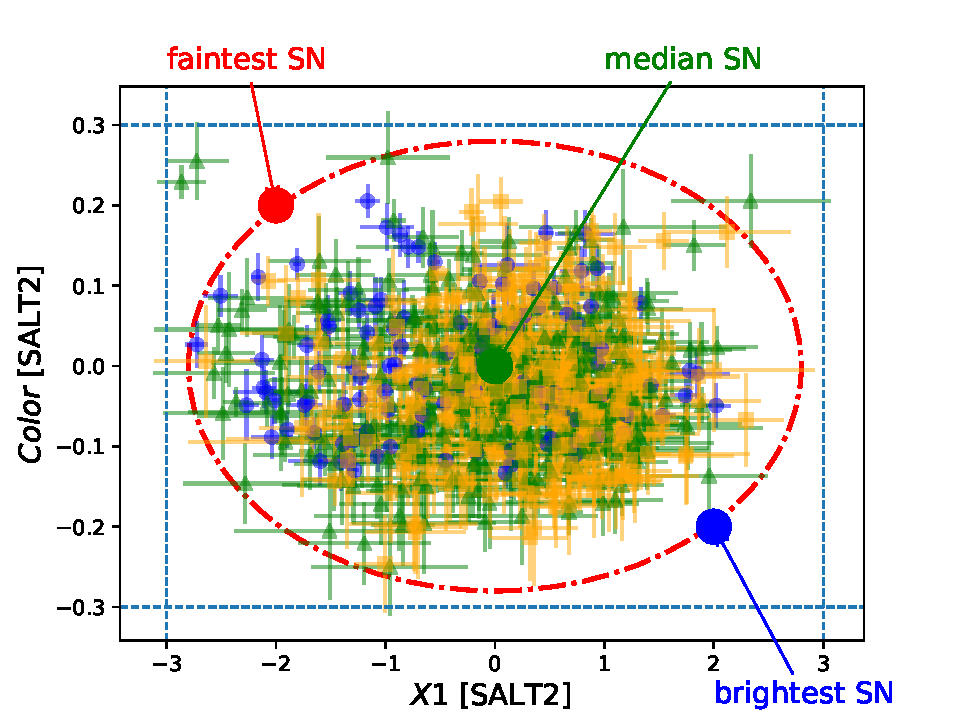
\includegraphics[width=0.6\textwidth]{key_design/sn_parameter_space.pdf}
    \caption{JLA supernovae the $(X_1,Color)$ parameter space --
      (blue: nearby, green: SDSS, orange: SNLS).  The large dots
      indicate the position of the faint, median and bright fiducial
      SNe used for the cadence analyses.}
    \label{fig:jla_X1_C}
  \end{center}
\end{figure}

On the same figure, we have represented three fiducial SNe of
particular interest: the red dot represents the faintest SN in this
region of the parameter space $(X_1=-2, C=0.2)$, the green dot and
blue dots show the average $(X_1=0, C=0)$ and brightest SN $(X_1=2,
C=-0.2)$ respectively.

We can define the redshift limit \zfaint as the limit beyond which the
faintest fiducal SN no longer passes the light curve requirements. By
doing this, we ensure that all SNe that live in the fiducial $(X_1,C)$
parameter space and are below \zfaint do pass our light curve
requirements.  \zfaint defines a {\em redshift-limited sample} whose
selection function does not depend on the SN properties.

We can also define a similar limit, using the median supernova,
instead of the faint one.  This defines a SN sample whose upper
redshift bins are affected by a selection bias, which must be
determined using a simulation -- which itself depends on our knowledge
of the SN luminosity distribution at those redshifts.  The uncertainty
affecting the determination of the selection function generally limits
the usefulness of the redshift bins affected by a selection bias.
Since the selection function is generally symmetric around its 50\%
point, the size of the sample limited by \zmed gives a good
approximation of the total number of LSST SNe that will have precise
distances.


\subsection{Metrics}
\label{sec:metrics}
We propose to use as our primary metrics the size and depth of the
subset of well sampled SNe.  More precisely, we estimate, for each
cadence, the following quantities:

\begin{itemize}
\item the sample redshift limit, \zfaint defined above, and the number
  of well sampled supernovae below the redshift limit \nsnfaint
\item the redshift \zmed at which the median supernova defined above
  no longer passes the signal-to-noise requirements, and the number of
  well-sampled supernovae below this redshift, \nsnmed.  
\end{itemize}
The former give an assessment of the size and depth of the redshift
limited sample, i.e. the sample of supernovae usable for cosmology,
and whose selection function is extremely easy to determine.  The
latter gives an assessment of the size and depth of the sample of SNe
that will have precise distances.



\section{Overview of observing strategies}


\subsection{Available strategies}

Four classes of observing strategies have been studied in detail:
\begin{itemize}

\item the {\tt OpSim}-based cadences released along with the white
  paper call (11 cadences released in June 2018 plus 4 additional
  simulations released in August), 
  
\item the {\tt OpSim}- and {\tt Feature}-based strategies that were
  available before the white paper call. 

\item simulations based on the {\tt Altsched} scheduler proposed by
  Stubbs and Rothchild.  This includes one rolling and another
  non-rolling cadence, plus a non-rolling simulation conducted on a
  larger footprint (P. Gris),

\item finally, we have tested a series of experimental observing
  strategies, based on the new feature-based scheduler (a.k.a.  SLAIR,
  Yoachim et al). These variations were produced by P. Yoachim, the
  main author of SLAIR, based on discussions we had at the summer 2018
  DESC week (CMU) and the 2018 LSST community workshop (Tucson).
\end{itemize}

In table \ref{tab:global_cadence_stats} we report, for each cadence
the total number of exposures per filter. This gives a general idea of
the total open shutter time, and the global filter allocation.  In
table \ref{tab:sn_specific_cadence_stats}, we show SN-specific key
statistics, in particular, the median number of visits in each filter,
for a given location of the sky (e.g. a healpixel), the median cadence
delivered by the observing strategy, the median season duration and
the total footprint of the survey.

The DDF  observations involve a  small number of fields  and $O(10^4)$
SNe. The list of simulated DDF is given in table
\ref{tab:ddf_list} and on figure \ref{fig:ddf_map}. The location of four DDF (referred to as reference fields in the following: \cosmos, \xmmlss, \cdfs~and \elais) has already been chosen by the project. The number of considered DDF ranges from 4 to 9.


\begin{table*}[!htbp]
  \begin{center}
  \begin{tabular}{|l|c|c|c|c|}
    \hline
    Field name & OpSim ID & Ra (deg) & Dec(deg) & Observing strategies\\
    \hline
    \cosmos & 2786 & 150.36 & 2.84 &All \\
    \xmmlss & 2412 & 34.39 & -5.09 & All \\
    \cdfs & 1427 & 53.00 & -27.44 & All \\
    \elais & 744 & 0.  & -45.52 & All \\
    \spt & 290 & 349.39 & -63.32 & All except feature*\\
    \ddfa & 820 & 119.55 & -43.37 & kraken\_2035\\
    \ddfb & 858 & 187.62 & -42.49 & kraken\_2035\\
    \ddfc & 1200 & 176.63 & -33.15 & kraken\_2035\\
    \ddfd & 2689 & 201.85 & 0.93 & kraken\_2035\\
    \hline
  \end{tabular}
  \caption{List and location of Deep Drilling Fields observed. "All" stands for all simulations but the ones performed with altsched.}\label{tab:ddf_list}
  \end{center}
\end{table*}


\begin{figure}[htbp]
\begin{center}
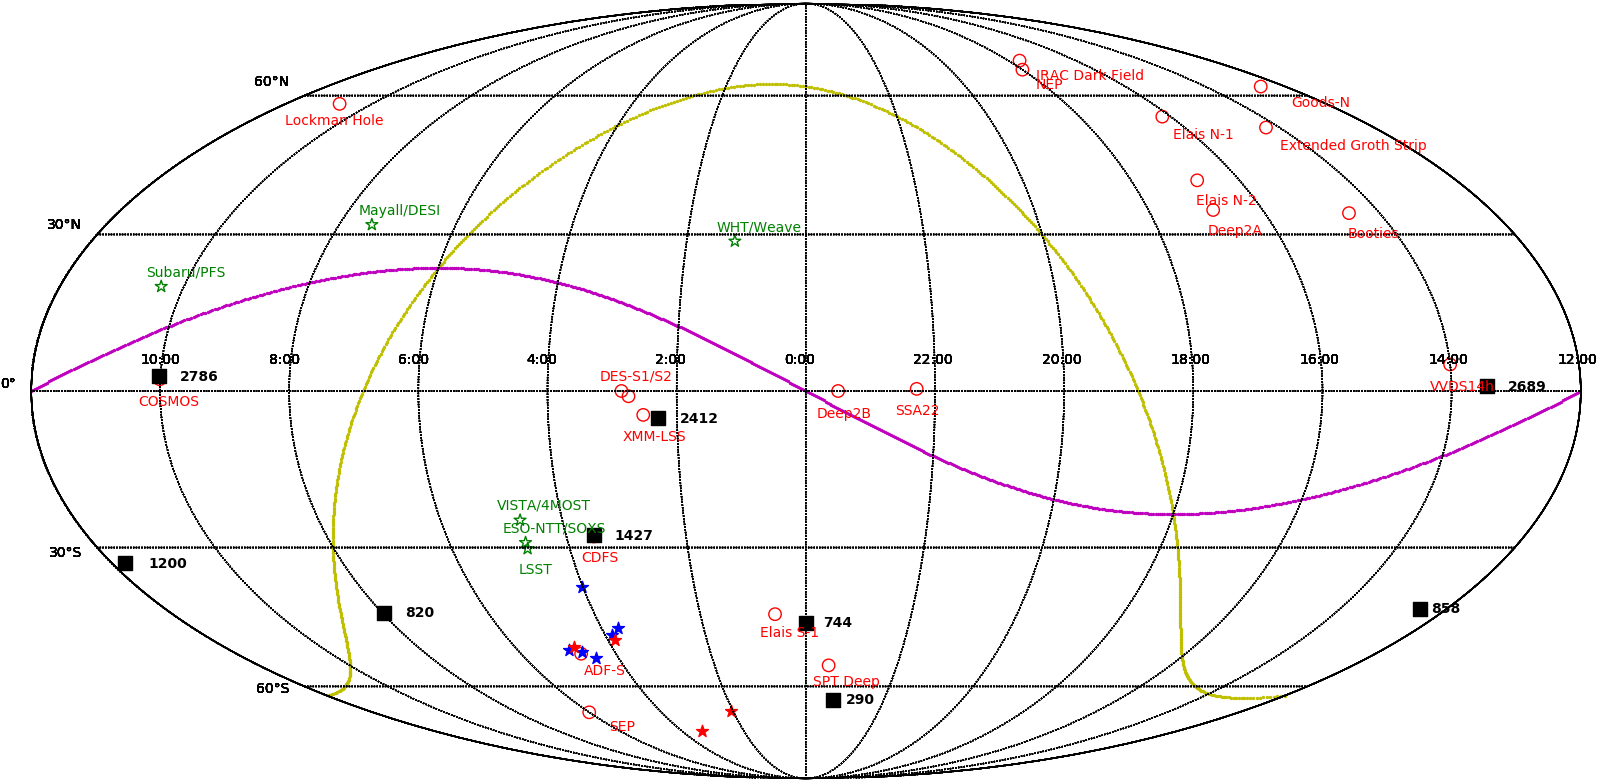
\includegraphics[width=14cm,height=10cm]{overview_strategy/All.png}
\caption{Location of the Deep Drilling fields observed (black squares). Deep fields observed by previous surveys (red circles) and potential candidates for spectroscopic follow-up (green stars) are also mentioned. Yellow and magenta lines represent the Galactic and Ecliptic planes, respectively. Blue and red stars indicate potential deep field locations for EUCLID and WFIRST, respecivelly.}\label{fig:ddf_map}
\end{center}
\end{figure}

DDF observations are composed of sequences of 96 visits (in a row) in r,g,i,z,y bands (namely 20,10,20,26,20 visits). This corresponds to a total observing time of about one hour and few minutes if filter changes, slew times and telescope overheads are taken into account.

\subsection{Key properties}

\subsubsection {WFD}
\label{sec:wfd_cadence_key_properties}

\paragraph{Effective SN cadence} What ultimately determines the quality of the SN light curves
and distances is the {\em effective} cadence delivered by the survey,
i.e.  the cadence evaluated after having stacked all the same-band
revisit pairs (or sometimes triplets) performed during one single night. The cadence may be estimated, on each
healpixel, by computing the mean time interval between visits -- after
having excluded the long duration gaps when the healpixel is not
observable.

The effective cadence varies considerably from one observing strategy
to another.  As an illustration, we present on figures
\ref{fig:pontus_2502_effective_cadences},
\ref{fig:altsched_effective_cadences} and
\ref{fig:altsched_rolling_effective_cadences}, we present effective
cadence maps for {\tt Pontus\_2502}, {\tt altsched} and {\tt altsched
  rolling} strategies.  On figure \ref{fig:effective_cadence}, we
report the median cadence in $r$ (computed from similar maps).  The
best effective cadences are delivered by the \altsched like
strategies. We note that there is about a factor 7 between the best
and worst effective cadences.

\begin{figure}
  \begin{center}
    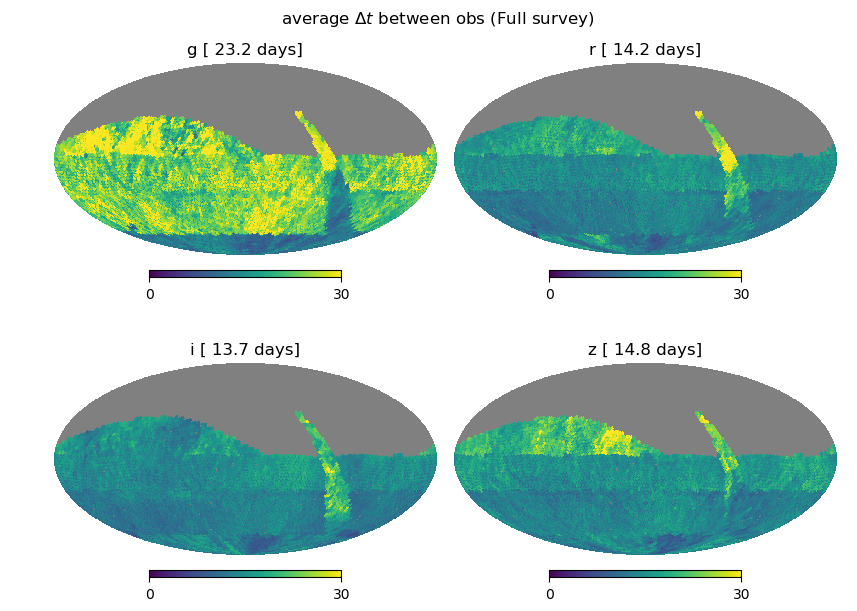
\includegraphics[width=0.8\linewidth]{overview_strategy/pontus_2502_cadence.png}
    \caption{Average $\Delta T$ between observations for {\tt
        Pontus\_2502}, a (slightly rolling) strategy that implements
      same-band visit pairs. }
    \label{fig:pontus_2502_effective_cadences}
  \end{center}
\end{figure}


\begin{figure}
  \begin{center}
    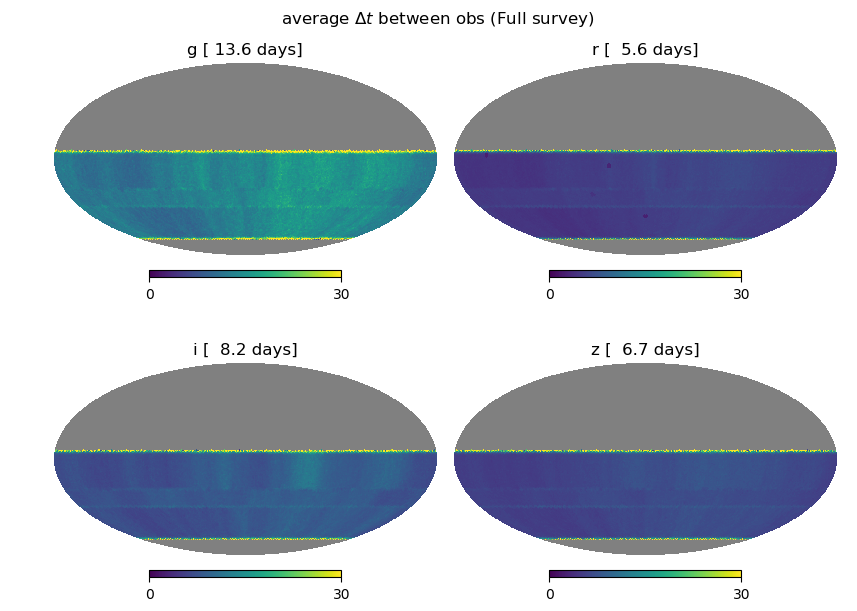
\includegraphics[width=0.8\linewidth]{overview_strategy/altsched_cadence.png}
    \caption{Average $\Delta T$ between observations for {\tt
        Altsched}, a strategy that avoid same band visit pairs.}
    \label{fig:altsched_effective_cadences}
  \end{center}
\end{figure}


\begin{figure}
  \begin{center}
    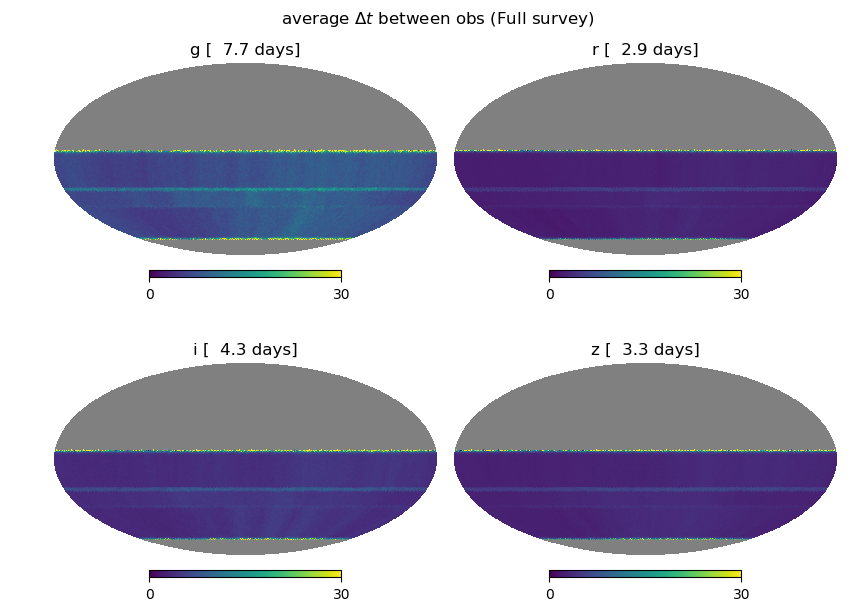
\includegraphics[width=0.8\linewidth]{overview_strategy/altsched_rolling_cadence.png}
    \caption{Average $\Delta T$ between observations for {\tt
        Altsched} rolling, a rolling strategy that avoids same band
      visit pairs.}
    \label{fig:altsched_rolling_effective_cadences}
  \end{center}
\end{figure}

\begin{figure}
  \begin{center}
    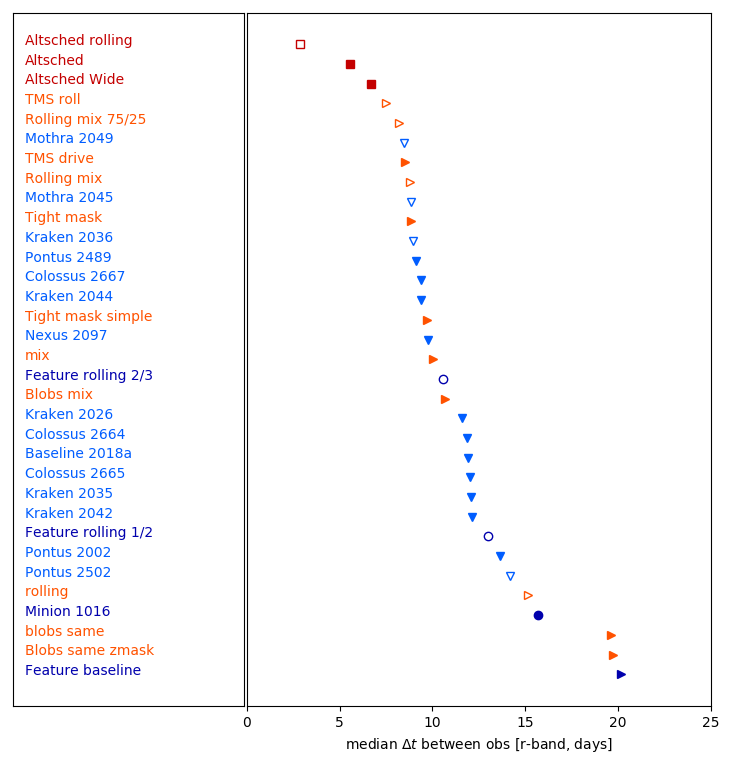
\includegraphics[width=0.8\linewidth]{overview_strategy/cadence.png}
    \caption{Assessment of the effective SN cadence for all
      strategies: median $\Delta T$ between observations (after
      grouping same night observations). \altsched cadences are shown
      in red, \opsim cadences released for the white paper call in
      blue, \slair in orange, and early cadences in deep blue. The
      rolling (resp. non-rolling) cadences are displayed with open
      (resp. solid) markers. }
    \label{fig:effective_cadence}
  \end{center}
\end{figure}

In the remaining of this section, we discuss some of the key design
elements that can explain such large differences.


\paragraph{Global filter allocation} All \opsim and \slair cadences   share the same global filter balance: 
$\sim 7\%, 10\%, 22\%, 22\%, 21\%$ and $18\%$ of the total open shutter time
are allocated to the $u, g, r, i, z$- and $y$ bands respectively.
\altsched makes a different choice, based on the fact that the
low-throughput of the LSST camera in $y$, combined with the high sky
brightness in that band limit the impact of $y$-band observations.
About half of the $y$-band observing time is therefore reallocated to
$g$, $r$ and $i$ and $z$ bands, the resulting filter balance is
therefore: 9\%, 11\%, 28\%, 18\% 26\% and 9\% ($ugrizy$ respectively). Of course, having more
observing time in $griz$ can only improve the quality of SN~Ia light curves and distances.


\paragraph{Filter allocation strategy} Another key point, is how the filters are
changed during the night.  In this regard, very different strategies
have been implemented by the various schedulers proposed so far.  This
is illustrated on figure \ref{fig:hourglass_plot_filter_alloc}, which
shows the filter usage for  {\em Pontus 2002} and {\em
  AltSched rolling}.  {\em Pontus 2002} attempts to minimize the
filter changes during a night and in fact keeps observing in the same
filter over several nights.  Conversely, the \altsched family of
cadences attempt to switch for a different filter after each observing
block, so that each revisit of the same field is performed in a
different band.  As we will see below, this has a major impact on the effective cadence
delivered by the survey. As of today, most \opsim cadences released so
far try to minimize the number of filter changes, all \altsched cadences
switch filters after each observing block, and \slair has been
experimenting with both strategies.

\begin{figure}
  \begin{center}
    \subfigure[Pontus 2002]{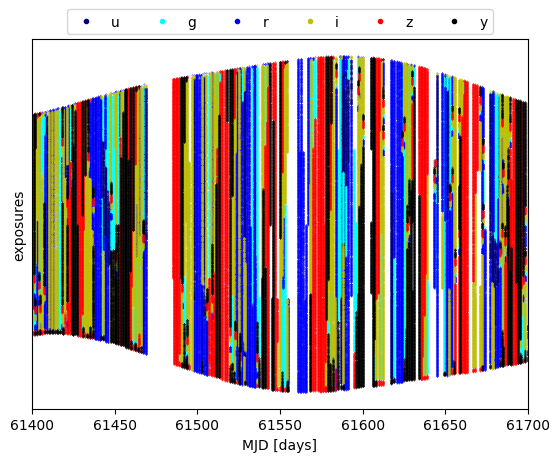
\includegraphics[width=0.48\linewidth]{overview_strategy/pontus_2002_hourglass.png}}
    \subfigure[AltSched rolling]{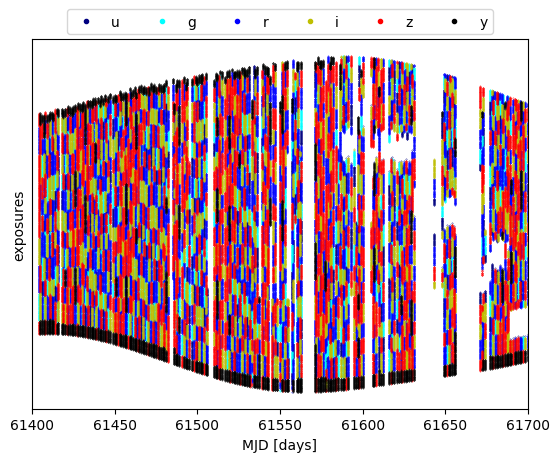
\includegraphics[width=0.48\linewidth]{overview_strategy/alt_sched_rolling_hourglass.png}}
    \caption{Hourglass plots showing the filter usage for two
      different observing strategies. Most \opsim and \slair observing
      strategies released so far tend to minimize the number of filter
      changes. The AltSched strategy makes sure that each field is
      observed twice a night in different filter. This results in a
      higher number of filter changes, but is highly beneficial for
      the SN follow-up. }
    \label{fig:hourglass_plot_filter_alloc}
  \end{center}
\end{figure}

\paragraph{The combined effet of visit pairs and filter allocation strategy} In all cadences proposed so far
(except a few simulations, notably {\tt colossus\_2667} and {\tt
  kraken\_2044}) all fields are observed twice a night, 1 to 2 hours
apart, in order to improve the detectability of short term transients
and solar system objects.  Depending on the filter allocation
strategy, this has a strong impact on the sampling quality of the
SN~Ia light curves.  Indeed, SN~Ia luminosities vary significantly
over time scales of 1-2 days.  Same band observations taken during a
given night may therefore be considered as one single visit. When
dealing with a fixed total number of visits per sky direction,
re-observing a field in the same band during a night degrades the SN
light curve sampling by a factor $\sim 2$.

\begin{figure}
  \begin{center}
    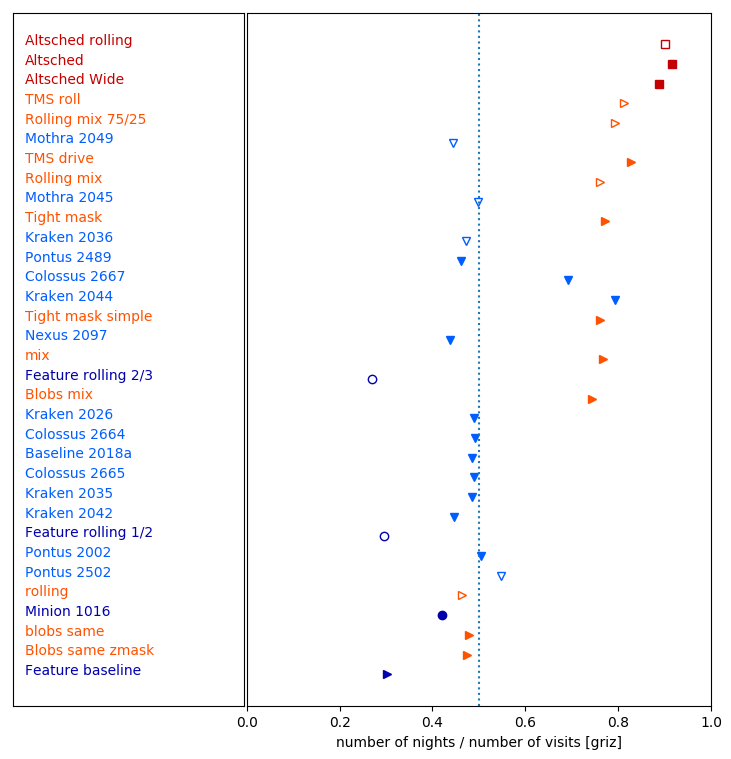
\includegraphics[width=0.8\linewidth]{overview_strategy/night_visit_ratio.png}
    \caption{Number of nights vs. number of visits for the median
      healpixel. We clearly see the effect of the same-band revisit
      strategy.  \altsched cadences are show in red, \opsim WPC in
      blue, \slair in orange, and early cadences in deep blue. The
      rolling (resp. non-rolling) cadences are displayed with open
      (resp. solid) markers. }
    \label{fig:effective_number_of_visits}
  \end{center}
\end{figure}

To estimate that, we compute, for each cadence, the healpix maps
giving the total number of {\em visits} per pixel and the total number
of {\em nights} (several visits per night).  On figure
\ref{fig:effective_number_of_visits}, we show, for each cadence, the
ratio of the median of these maps.  

The survey strategies are sorted according to the effective $r$-band
cadence delivered by the survey (see figure
\ref{fig:effective_cadence}).  We note that most good-cadence
strategies avoid same band revisit pairs. Some strategies however, are
able to compensate.  These are either rolling strategies ({\tt
  Mothra\_2049}, {\tt Mothra\_2045} or {\tt Kraken\_2036}) or by
increasing the total number of visits ({\tt Pontus\_2489}).

All \opsim cadences, except {\tt colossus\_2667} and {\tt
  kraken\_2044} the number of visits is about twice the number of
distinct nights, which is likely to degrade the effective SN cadence
(deeper visits, less often).  All \altsched simulations attempt to
avoid this, as do the recent experiements conducted with \slair.

\paragraph{Season length} This is another feature that may alter the cadence, and the size of the SN sample.
Nearby supernova light curves are less
affected by redshift time dilation, so season duration is not as
crucial as for DDF observations.  However, it is a quantity worth
estimating, in particular to see whether it correlates with the
effective cadence and/or the total size of the SN sample.
Figure \ref{fig:season_length} shows the average season length for
each cadence studied in this work (sorted by $r$-band effective
cadence).  We see considerable differences in season durations (from 130 to 200 days).
Most \opsim and all \altsched strategies manage to observe each field during about
150 consecutive days. The shorter (130 days) and longer (170 days) seasons come mainly from  \slair 
for reasons that have not been elucidated yet. In any case, we do not
note any significant correlation between season duration and cadence.

\begin{figure}
  \begin{center}
    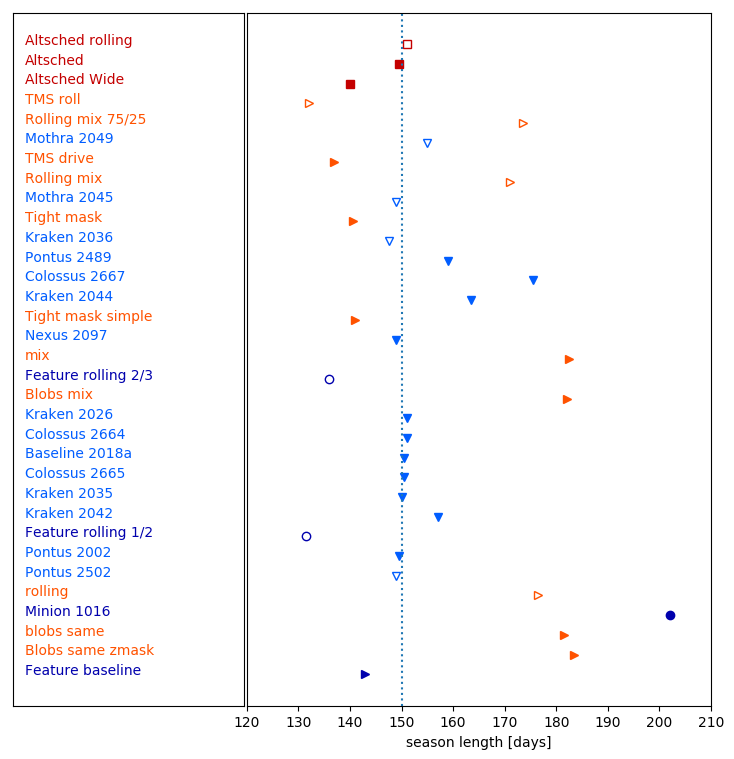
\includegraphics[width=0.8\linewidth]{overview_strategy/season_length.png}
    \caption{Median season duration for each cadence in this
      study. \altsched cadences are show in red, \opsim WPC in blue,
      \slair in orange, and early cadences in deep blue. The rolling
      (resp. non-rolling) cadences are displayed with open
      (resp. solid) markers. }
    \label{fig:season_length}
  \end{center}
\end{figure}


\paragraph{} To conclude: we note a very large gap (about a factor 7) between
the best and the worst cadences delivered by the various strategies
released so far.  We will see in the next section, that effective
cadence is the key to maximize the size and depth of the SN sample.
We have discussed a few design elements that help improving the effective
cadence: (1) implementing a rolling strategy (2) change filters often
during the night (3) avoid same band visit pairs.

However, each of these elements taken alone is not
sufficient. Combining all of them has been tried, for example in the
\slair cadences {\tt tms\ roll} and {\tt rolling mix*} and has brought
tremendous improvements with respect to the previous experiments
conducted with this scheduler.  However, the best \slair simulations
are still behind \altsched regarding cadence.  On top of the elements
discussed above, the core of the \altsched observing strategy ensures
an extreme regularity of the cadence.

\FixMe{nrl, 2018-09-27: we still need to estimate (1) the same-filter
  1-day gaps (2) the cadence rms. I think that would help
  understanding the difference between the best SLAIR cadences and
  Altsched. }.



\subsubsection{DDF}


All proposed observing strategies but altsched-like have included DDF.
Plots illustrating the four key points mentioned above are given on Figures \ref{fig:cosmos_cad}-\ref{fig:spt deep_m5} for baseline18a, feature\_baseline\_10yrs, kralen\_2026 and kraken\_2035 observing strategies and for the five to nine above-mentioned DDF. Among these cadences feature\_baseline\_10yrs displays interesting features with respect to supernovae observations for the reference DDF:

\paragraph{Cadence} a median cadence of three days is observed whereas other observing strategies present cadences that may reach up to 14 days. Inter-night gaps are also smaller for \cosmos~and \xmmlss: 10 to 15 days and 5 to 7 days for the first and second maxima respectively whereas  for baseline18a, kralen\_2026 and kraken\_2035 the first (second) maximum is at the level of 18 to 40 (13 to 20) days.  

\paragraph{Season length} feature\_baseline\_10yrs shows the highest season lengths with values around 150 days for \cosmos~and \xmmlss, and 180 days for \cdfs and \elais whereas other strategies lead to values of about 130, 140, 120, and 150 for \cosmos, \xmmlss, \cdfs, and \elais, respectively.

\paragraph{Depth} while median m5-values are compatible among the strategies (the decrease during season 2 for the four fields in  feature\_baseline\_10yrs is due to a known bug in the weather simulations) the coadded m5 depth per season shows clearly that feature\_baseline\_10yrs is a 0.7 (\cosmos), 0.4 (\xmmlss, \cdfs, \elais) magnitude deeper (r-band) survey compared to the others. This results is to be explained by better cadences and longer seasons.
 
Key properties of \spt, \ddfa, \ddfb, \ddfc~and \ddfb~fields are given on Figures \ref{fig:spt deep_cad} to\ref{fig:kraken_m5}.



\section{Metrics}

\subsection{Number of well-measured type \sne}

\subsubsection{Requirements on SN sampling}
\label{sec:sn_sampling_requirements}

Light curves are the essential ingredient to (1) measure standardized
luminosity distances and (2) photometrically identify SNe~Ia from
their full light curve. This drives a series of requirements which are
summarized below.

\begin{enumerate}

\item each SN must have good quality measurements in at least three
  bands. We need two bands, covering the restframe $B$ and $V$ region,
  to constrain the restframe color of the SN. We need to provision an
  additional band (redder than restframe $V$), to enable next
  generation standardization techniques, that will likely rely on two
  restframe colors.

\item the follow-up of each supernova must be good enough in the
  observer-frame bands that correspond to the $B$- and $V$-restframe
  spectrum ($3800 \angstrom < \lambda < 7000 \angstrom$).  At
  high-redshift, in particular, one should avoid relying on the $UV$
  restframe region to derive a distance, given the high intrinsic
  dispersion of SN~Ia at those wavelengths.
  
\item we require the light curve shape to be well sampled in the
  (restframe) phase interval $[-10;+30]$ days, with at least five
  visits before peak (each of those visits in any of the eligible
  band), and ten visits after peak.  To obtain this in the lower
  redshift region of the Hubble diagram, one requires an
  observer-frame cadence of 4 days.  At higher redshifts redshifts
  (DDF fields), this requirement may be slightly relaxed. However,
  since we are going to rely almost exclusively on photometric
  identification, it is essential to secure a tight sampling of the SN
  color evolution at all redshift.
  
\item we require that the photon noise contribution to the distance
  measurement is subdominant w.r.t. the intrinsic dispersion of the
  SNe (after standardization).  There are several ways to quantify
  this.  With today's standardization techniques, the SN standardized
  distance modulus is:
  \begin{equation}
    \mu = m^\star_B + \alpha X_1 - \beta C - \cal{M}
  \end{equation}
  where $m^\star_B$ is the peak brightness in restframe $B$, $X_1$
  characterize the lightcurve width, and $C$ is an estimate of the
  restframe color $B-V$. $\alpha$, $\beta$ and $\cal{M}$ are global
  parameters, fit along with the cosmology. If the light curve is
  correctly sampled (see point above), the propagation of the
  measurement uncertainties affecting $m^\star_B$, $X_1$ and $C$ is
  dominated by the contribution of $\sigma_C$. (since $\beta \sim
  3$). In practice, requiring $\sigma C < 0.04$ ensures that $\sigma
  \mu < 0.1$, below the intrinsic dipersion in the Hubble diagram,
  after standardization.
\end{enumerate}


\subsubsection{SN samples}\label{sec:metrics}

The SN sample usable for cosmology can be defined from the light curve
requirements listed in the previous section. A key quantity is the
redshift limit, $z_{lim}$, beyond which one starts loosing events
because of poor sampling.  This ``redshift-limit'' is not a
detectability limit.  It is the redshift value beyond which we start
losing a fraction of the events, because their photometric follow-up
does not match the requirements listed in the previous section.

The definition of the redshift limit depends on the intrinsic
luminosity of the supernova considered.  SN~Ia luminosities can be
parametrized using two parameters, e.g. lightcurve width ($X_1$) and
SN restframe B-V color at peak ($C$).  As shown on figure
\ref{fig:jla_X1_C}, the SN distribution in this parameter space is
compact and more than 95\% of the statistics can be enclosed in a
tight ellipse. 

\begin{figure}
  \begin{center}
    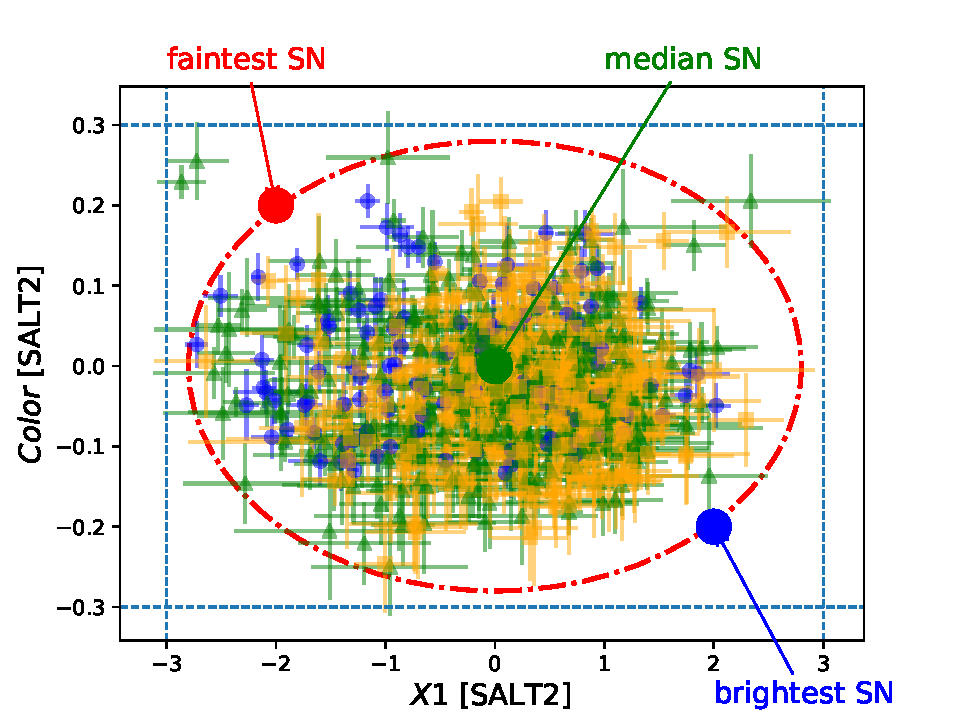
\includegraphics[width=0.6\textwidth]{key_design/sn_parameter_space.pdf}
    \caption{JLA supernovae the $(X_1,Color)$ parameter space --
      (blue: nearby, green: SDSS, orange: SNLS).  The large dots
      indicate the position of the faint, median and bright fiducial
      SNe used for the cadence analyses.}
    \label{fig:jla_X1_C}
  \end{center}
\end{figure}

On the same figure, we have represented three fiducial SNe of
particular interest: the red dot represents the faintest SN in this
region of the parameter space $(X_1=-2, C=0.2)$, the green dot and
blue dots show the average $(X_1=0, C=0)$ and brightest SN $(X_1=2,
C=-0.2)$ respectively.

We can define the redshift limit \zfaint as the limit beyond which the
faintest fiducal SN no longer passes the light curve requirements. By
doing this, we ensure that all SNe that live in the fiducial $(X_1,C)$
parameter space and are below \zfaint do pass our light curve
requirements.  \zfaint defines a {\em redshift-limited sample} whose
selection function does not depend on the SN properties.

We can also define a similar limit, using the median supernova,
instead of the faint one.  This defines a SN sample whose upper
redshift bins are affected by a selection bias, which must be
determined using a simulation -- which itself depends on our knowledge
of the SN luminosity distribution at those redshifts.  The uncertainty
affecting the determination of the selection function generally limits
the usefulness of the redshift bins affected by a selection bias.
Since the selection function is generally symmetric around its 50\%
point, the size of the sample limited by \zmed gives a good
approximation of the total number of LSST SNe that will have precise
distances.

For each cadence we may thus estimate the following quantities in addition to the total number of well-sampled supernovae: 

\begin{itemize}
\item the sample redshift limit, \zfaint defined above, and the number
  of well sampled supernovae below the redshift limit \nsnfaint
\item the redshift \zmed at which the median supernova defined above
  no longer passes the signal-to-noise requirements, and the number of
  well-sampled supernovae below this redshift, \nsnmed.  
\end{itemize}
The former give an assessment of the size and depth of the redshift
limited sample, i.e. the sample of supernovae usable for cosmology,
and whose selection function is extremely easy to determine.  The
latter gives an assessment of the size and depth of the sample of SNe
that will have precise distances.

\subsubsection{Deep Drilling fields}

\myparagraph{Method}

The strategy to estimate the number of well-measured type Ia supernovae may be summarized in four steps: (1) light curves are simulated and fitted using observations of a given cadence; (2) selection criteria are applied to get high-quality supernovae; (3) the resulting observing efficiency curves are then convolved with a production rate \cite{perrett} so as to estimate the number of well-measured type Ia supernovae that may be collected by LSST given an observing strategy. 

Table \ref{tab:sim_ddf} summarizes the parameter used in SN simulations. The selection of a sample of well-measured type Ia supernovae is done in two steps. A sample of observable supernovae is selected by requiring light curves to have \phasemin $\leq$ -5 and \phasemax $\geq$ 20 (where \phasemin~ and \phasemax~ are the minimal and maximum phases of the LC points, respectively). For each supernovae in this reference sample, additional selection criteria are applied:
\begin{itemize}
\item $N_{bef} \geq 4$ and $N_{aft} \geq 10$ where $N_{bef}$ and $N_{aft}$ are the number of LC points (with SNR$\geq$ 5) before and after \daymax.
 \item $\sigma_c \leq 0.04$ where $\sigma_c$ is the error on the \sncolor~parameter estimated from the fit of the light curve.
\end{itemize}
The season length which depends on the redshift is estimated using the supernovae of the reference sample.

\begin{table}[!htbp]
  \begin{center}
    \caption{Range of the parameters used to simulate type Ia SN}\label{tab:sim_ddf}
\begin{tabular}{cc}
  \hline
  \hline
Parameter & Range \\
\hline
\hline
                    & (-2.0,0.2),(0.0,0.0),(2.0,-0.2) \\
 (\strech,\sncolor) & (-2.0,0.0),(-2.0,0.2),(0.0,-0.2) \\
                    & (0.0,0.2),(2.0,0.0),(2.0,0.2) \\
\hline
\redshift           & [0.01,1.3] (step: 0.025) \\
\hline
\daymax             & [\tmin,\tmax] (step: 1 day) \\
                    & (\tmin~and \tmax~ are the min and max MJD of a season) \\
                    \hline
\end{tabular}
\end{center}
\end{table}

\myparagraph{Results}

Typical detection efficiencies are given on Fig. \ref{fig:effi} for the \cosmos~field and feature\_baseline\_10 yrs cadence . One may observe that the lowest efficiencies (independently on the (\strech,\sncolor) values) correspond to the first two seasons of observations which are known to be very bad for this observing strategy and for this field (see for instance Figs. \ref{fig:cosmos_cad} and \ref{fig:cosmos_m5}).

\begin{figure}[htbp]
\begin{center}
  
  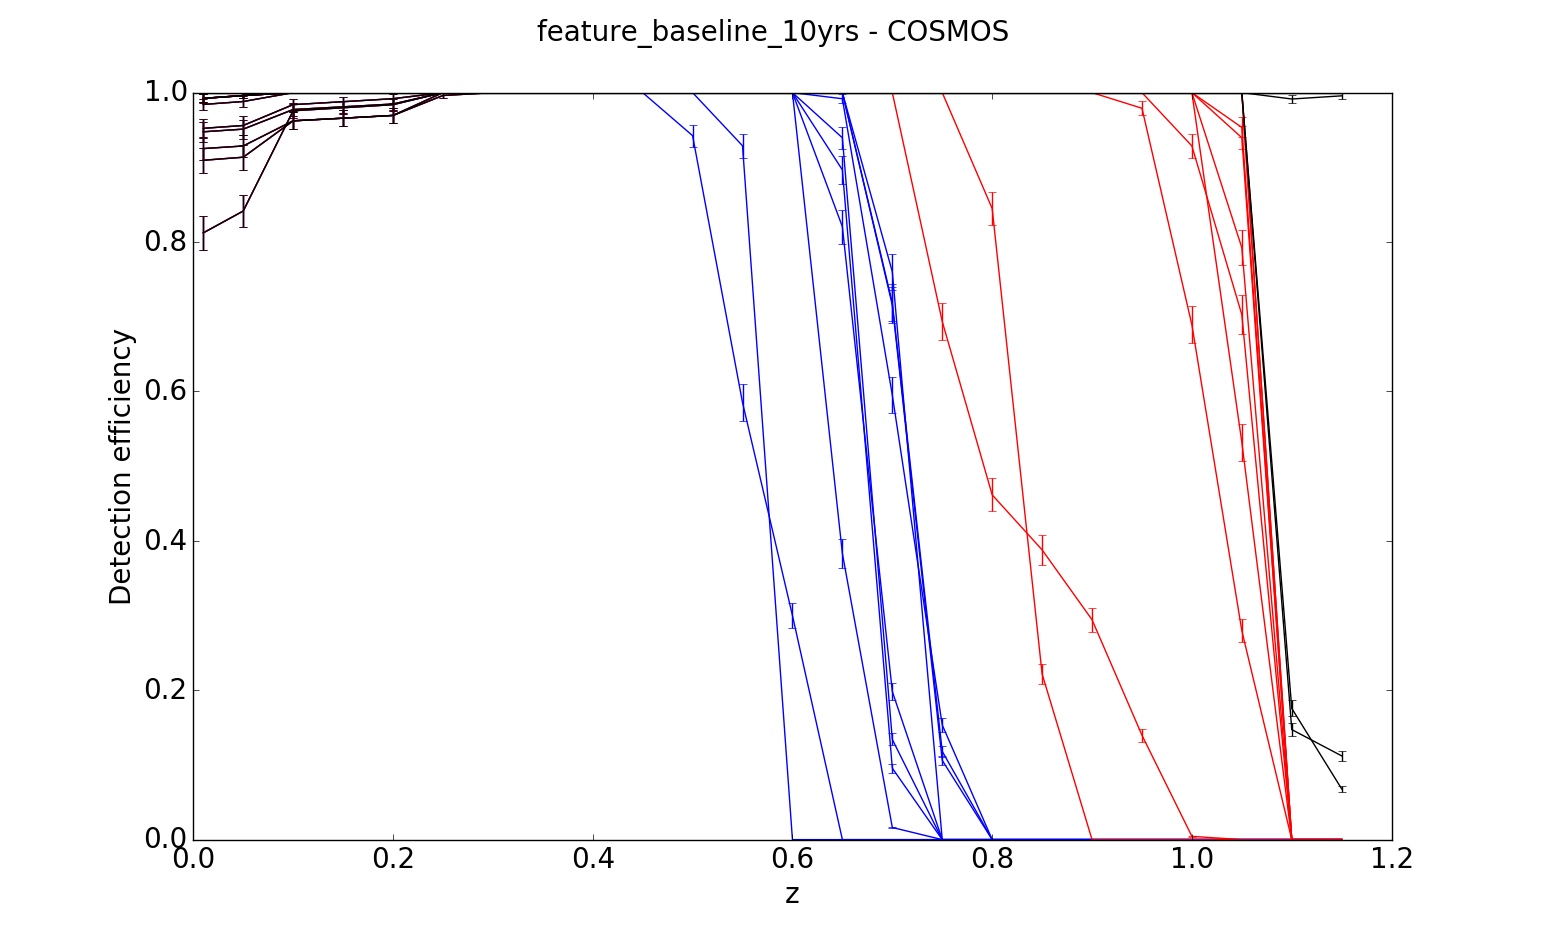
\includegraphics[width=12cm]{nsn/effi_feature_cosmos.png}
 \caption{Detection efficiency as a function of the redshift for the \cosmos~field and feature\_baseline\_10yrs observing strategy (10 seasons). Blue, red and black lines correspond to faint, medium and bright supernovae, respectively.}\label{fig:effi}
\end{center}
\end{figure}

Efficiency curves are convolved with a production rate \cite{perrett} to estimate the number of well-measured type Ia supernovae that may be collected by LSST. Summary plots are given for the reference fields (Fig \ref{fig:nsn_four}) and for all the DDF (Fig \ref{fig:nsn_all}). One may observe that, despite bad observing years, \feature~ shows the best results in terms of number of well-measured type Ia supernovae. Equivalent results are obtained with Colossus\_2667.

\begin{figure}[htbp]
\begin{center}
  
  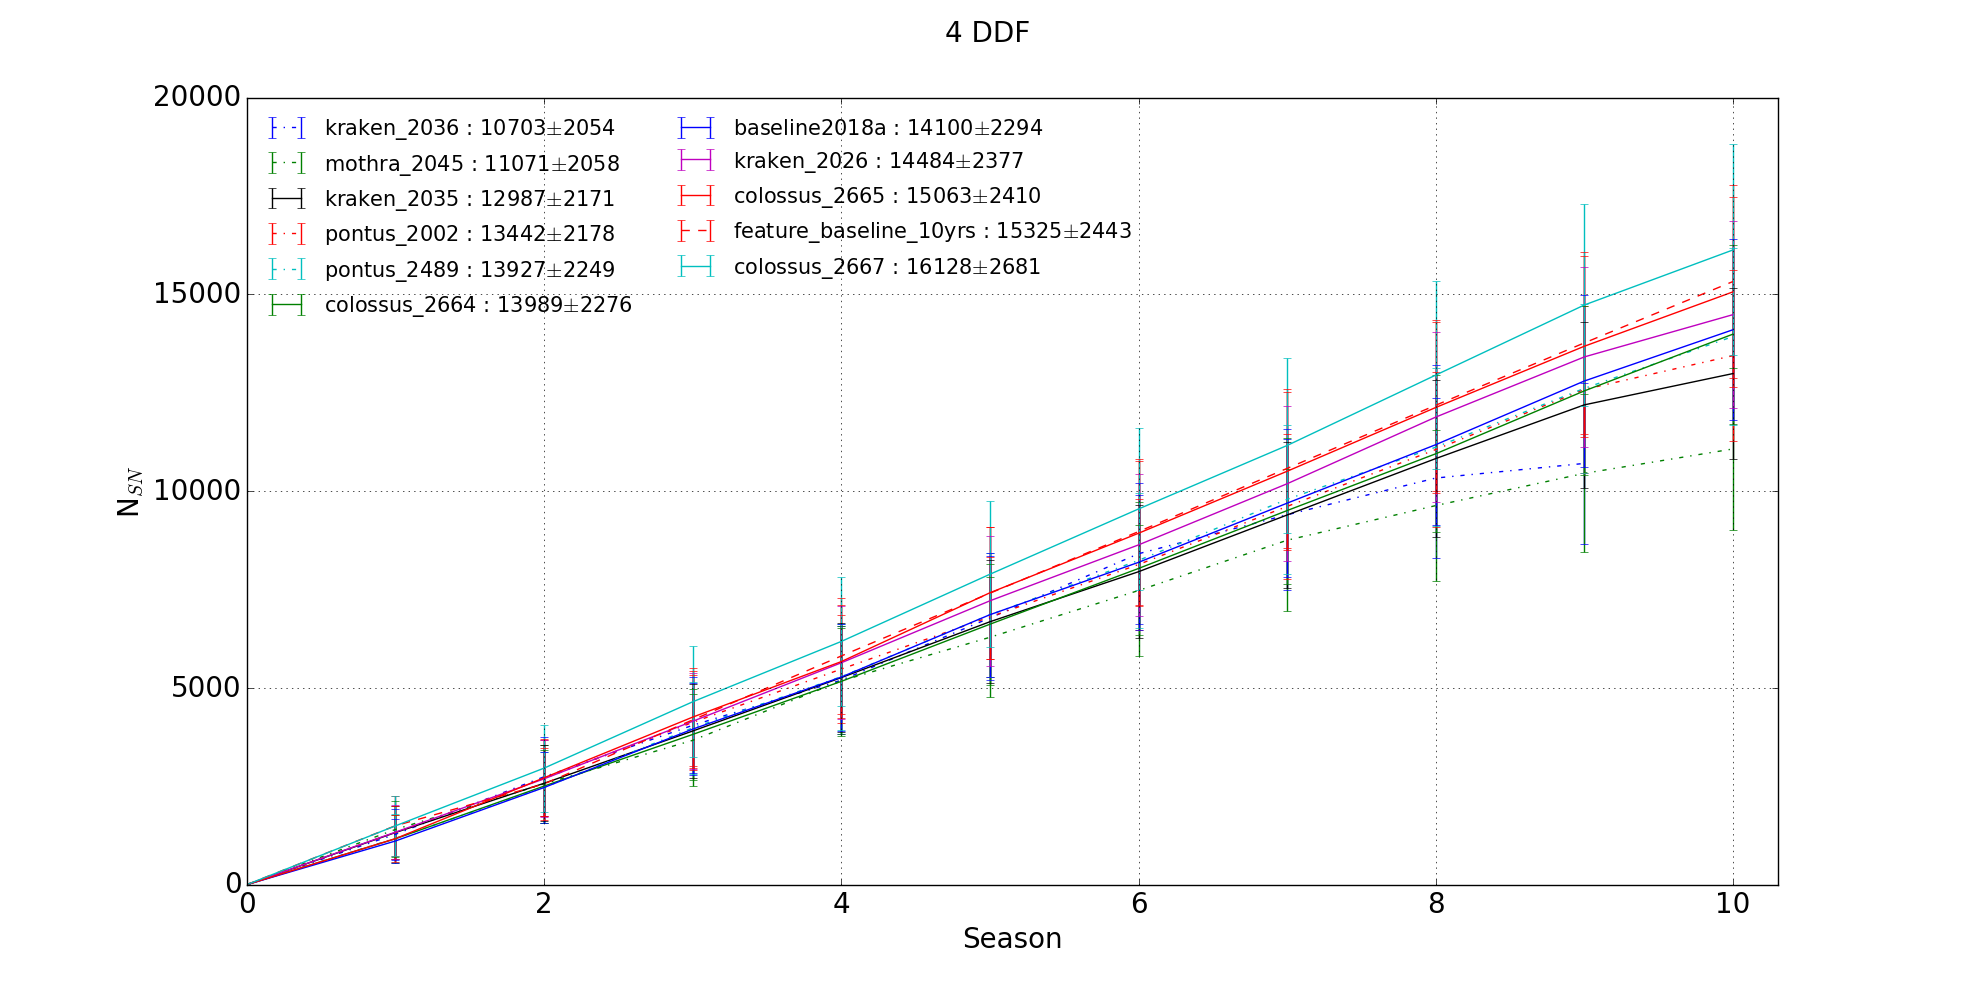
\includegraphics[width=15cm,height=10cm]{nsn/NSN_season_4DDF.png}
  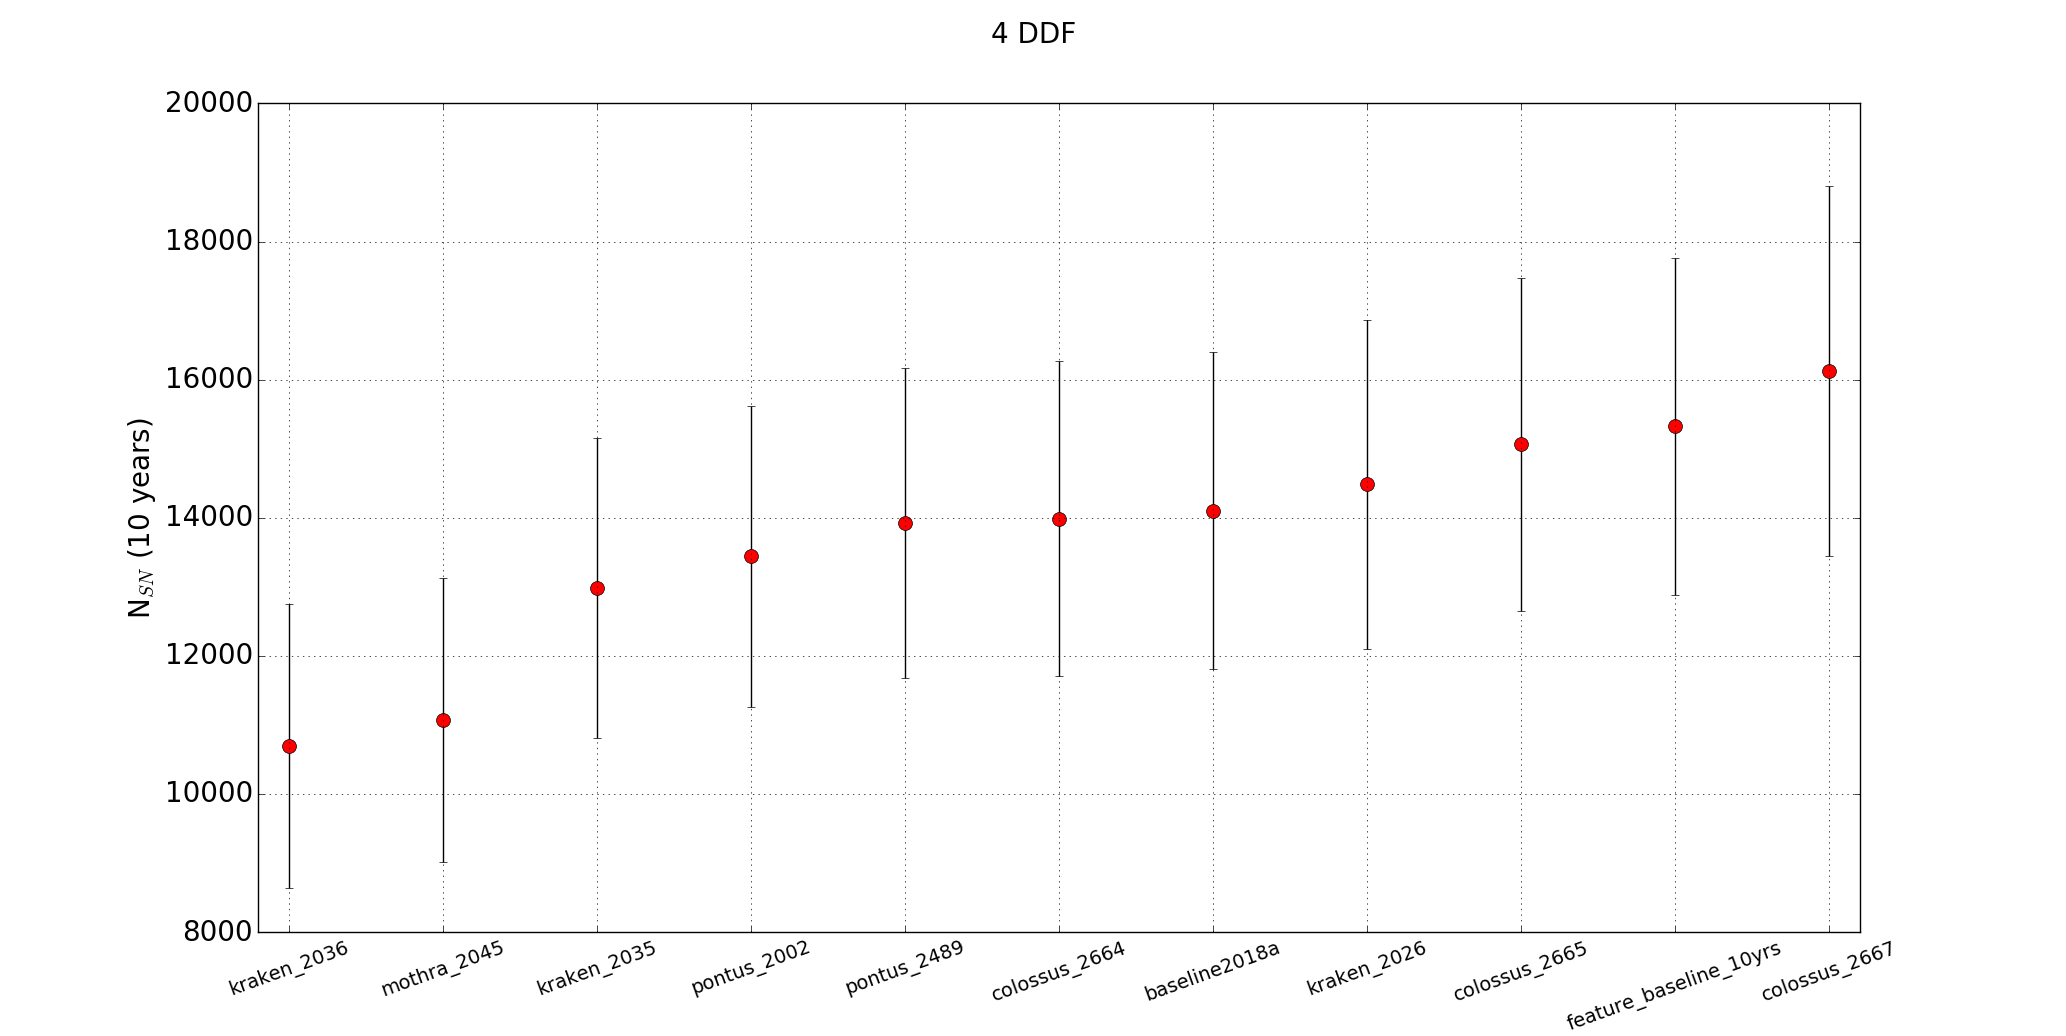
\includegraphics[width=15cm,height=10cm]{nsn/NSN_all_4DDF.png}
 \caption{Top: Number of well-measured type Ia supernovae as a function of the season. Bottom: Number of  well-measured type Ia supernovae as a function of observing strategy after ten years of operation. Four DDF (\cosmos,\xmmlss,\cdfs,\elais) have been considered.}\label{fig:nsn_four}
\end{center}
\end{figure}

\begin{figure}[htbp]
\begin{center}
  
  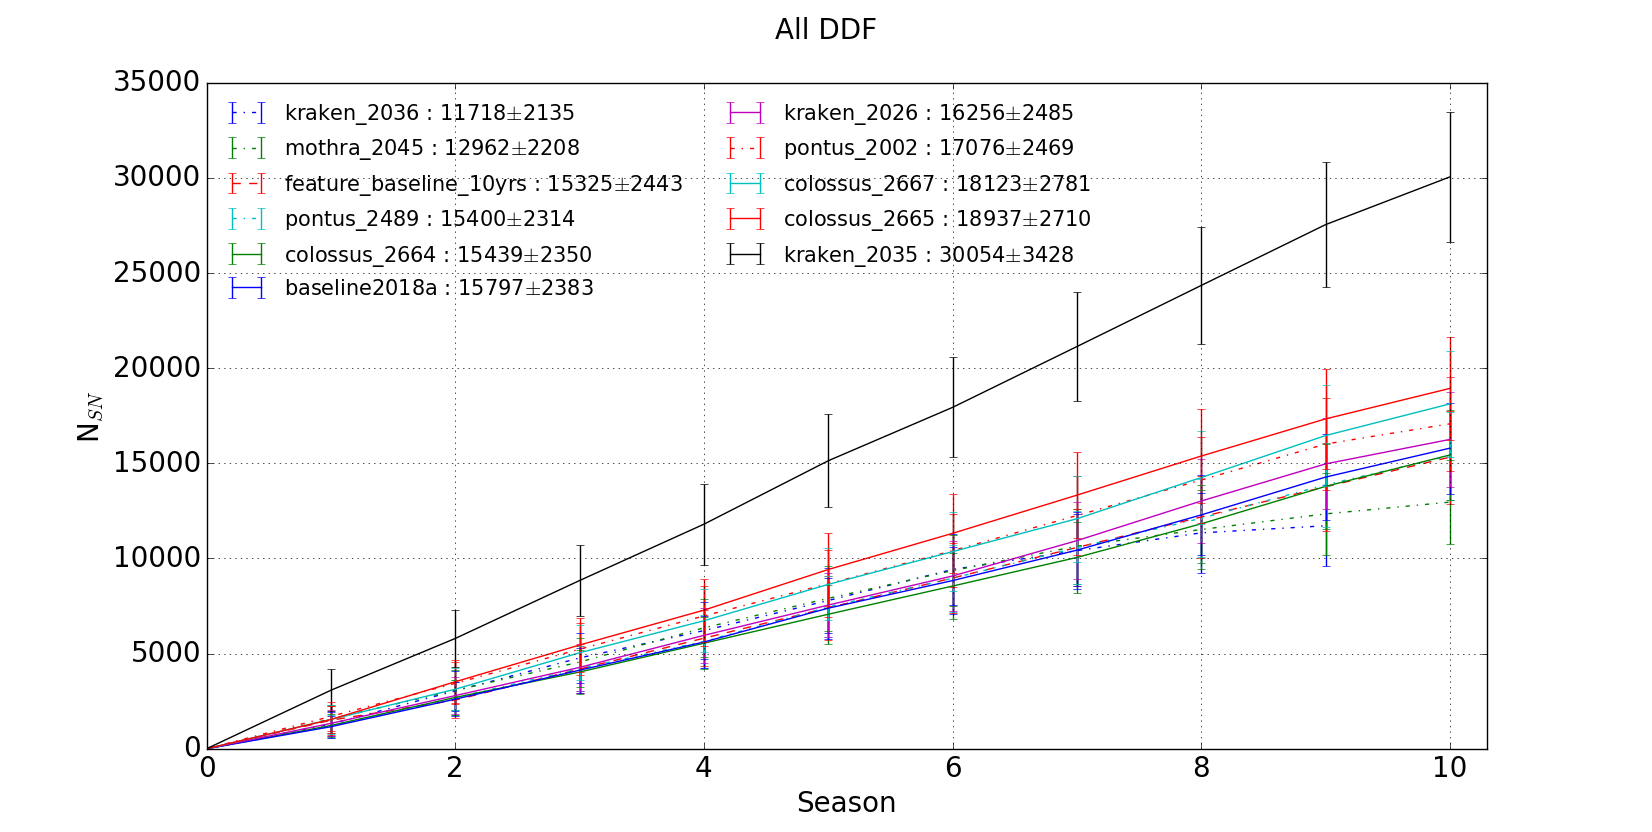
\includegraphics[width=15cm,height=10cm]{nsn/NSN_season_allDDF.png}
  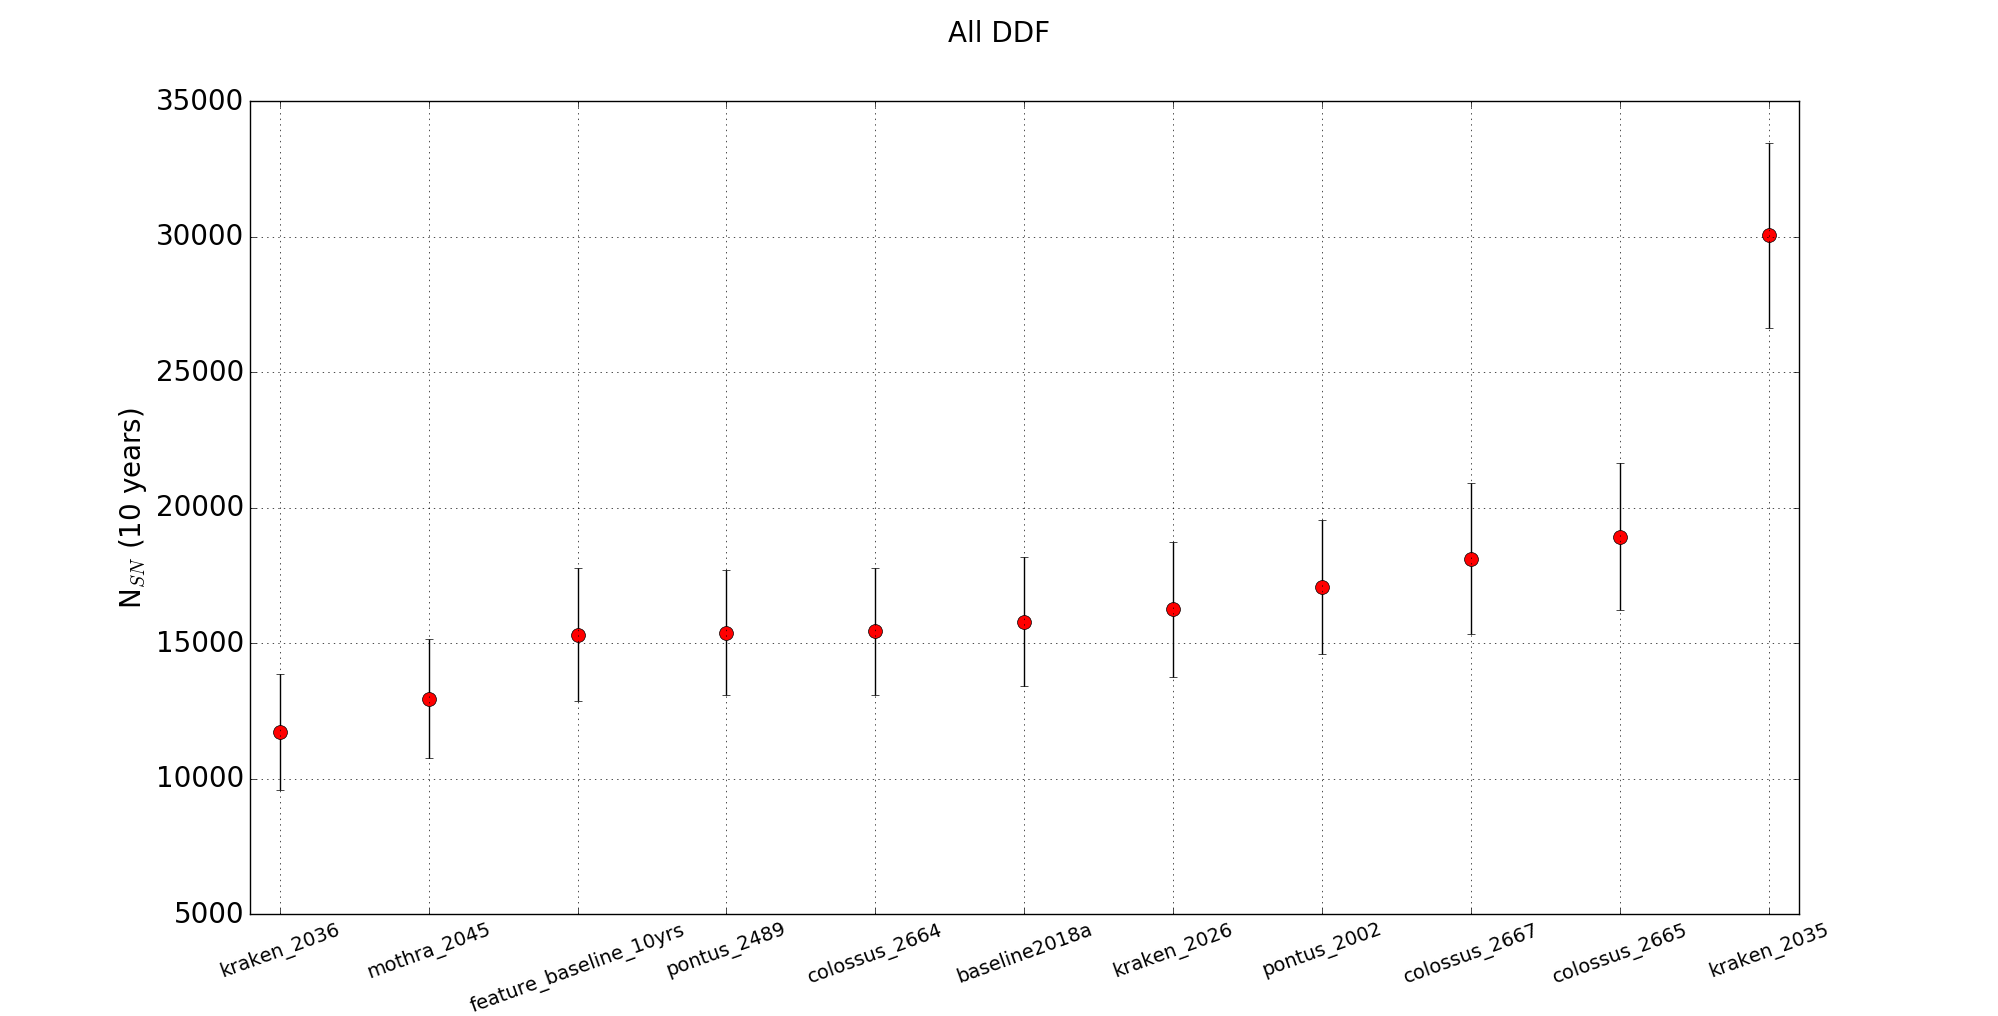
\includegraphics[width=15cm,height=10cm]{nsn/NSN_all_allDDF.png}
 \caption{Top: Number of well-measured type Ia supernovae as a function of the season. Bottom: Number of  well-measured type Ia supernovae as a function of observing strategy after ten years of operation. All DDF have been considered.}\label{fig:nsn_all}
\end{center}
\end{figure}

\myparagraph{Conclusion}

When considering all DDF the winner (w.r.t. the total number of well-sampled supernovae) is of course kraken\_2035 (30K after ten years) since this observing strategy considered 9 DDFs whereas all others observed 4 to 5 fields. One may observe that extrapolating a four fields configuration results (like the ones obtained with \feature) to a 9 DDF observing strategy will probably lead to an overestimation of the resulting number of well-measured type Ia supernovae. It is indeed difficult to maintain the same quality (in terms of cadence, season length and thus depth) when moving from a 4 to a 9 DDF strategy.

\begin{sidewaysfigure}
\begin{center}  
  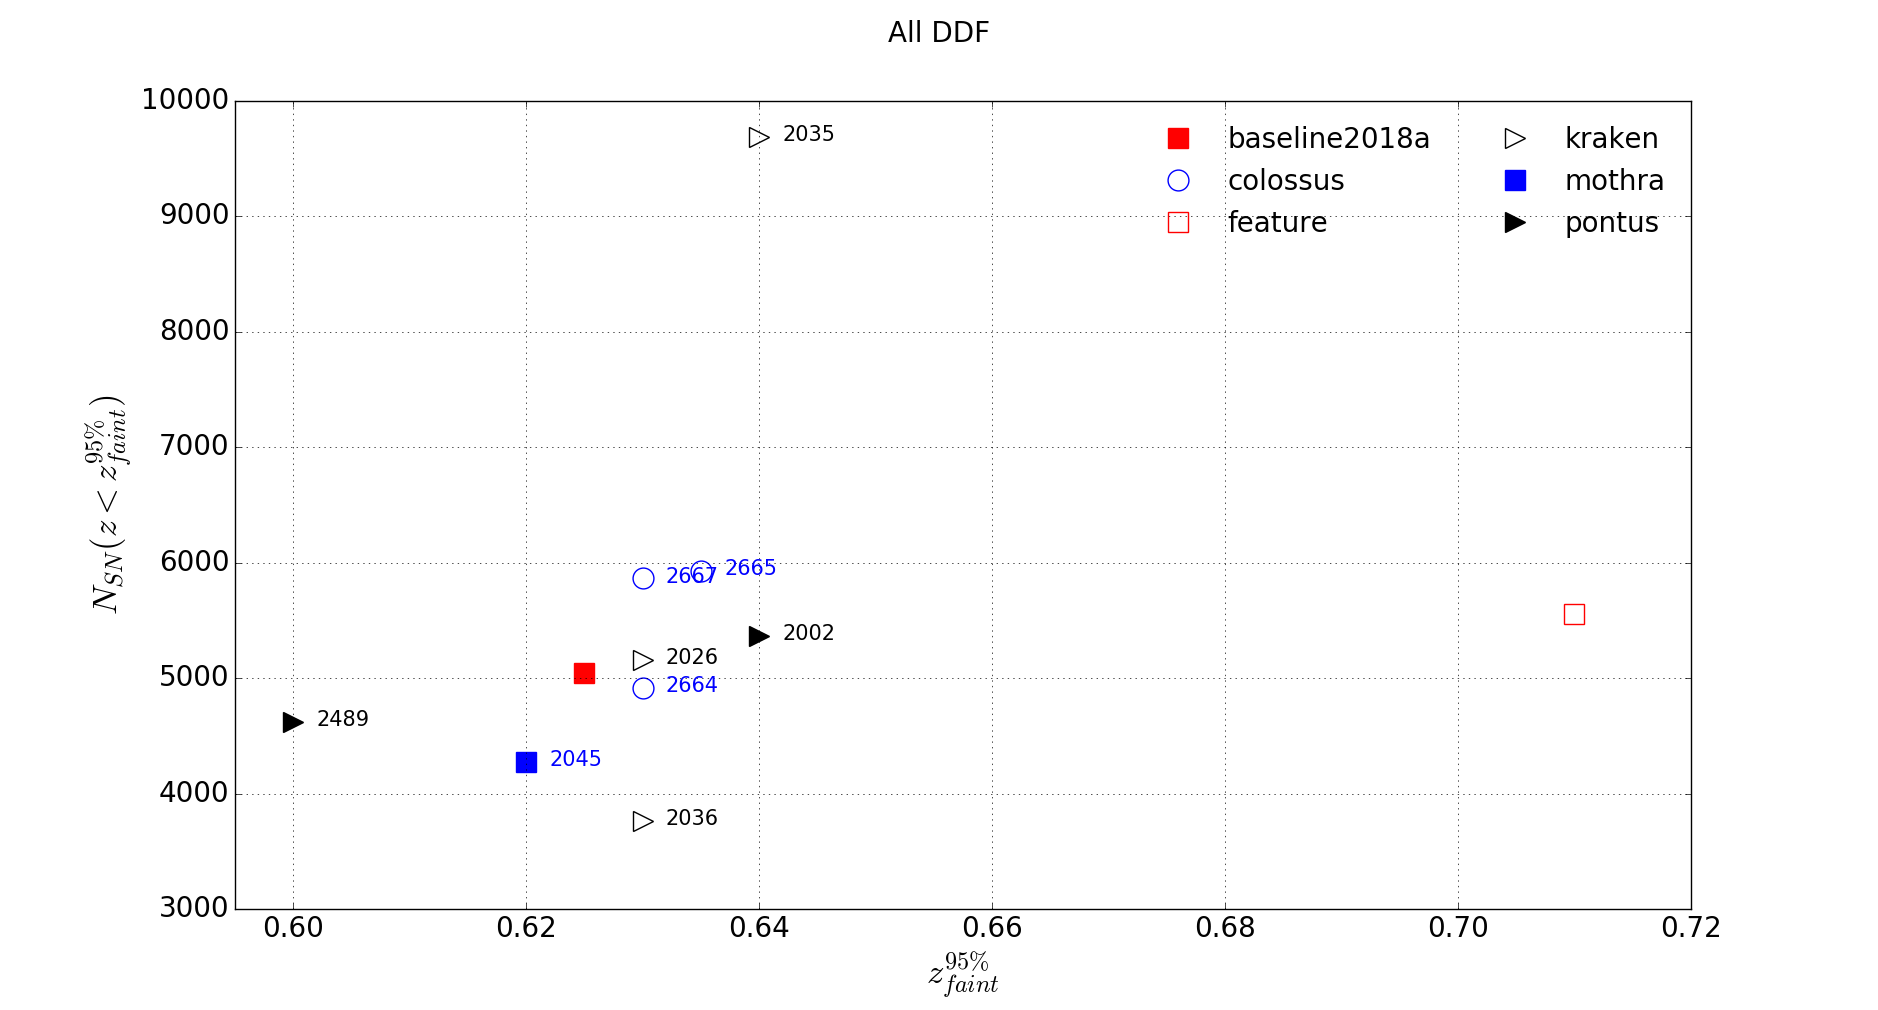
\includegraphics[width=\linewidth]{nsn/Z95_NSN.png}
 \caption{95\% redshift limit (ie corresponding to the detection of 95\% of the supernovae of the corresponding sample) as a function of the number of faint supernovae. Each point correspond to a field, a season and an observing strategy.}\label{fig:z95}
\end{center}
\end{sidewaysfigure}

Another way to assess the quality of an observing strategy is to estimate the redshift detection limit for faint supernovae (see \ref{sec:metrics}). On Figure \ref{fig:z95} is displayed the 95\% redshift limit (ie corresponding to the detection of 95\% of the faint supernovae sample) as a function of the number of faint supernovae. Huge variations among and inside strategies are observed. This plot reflects the quality of the proposed cadences. It seems that \redshift~of 0.7-0.75 may be reached with four fields. Once again \feature~tend to give the highest redshifts and the most homogeneous results among the fields and seasons. 


\subsubsection{Wide Fast Deep}
\label{sec:wide_fast_deep_analysis_method}

\myparagraph{Method}

WFD observations involve a large number of fields.  The observations
are dithered, and the size and depth of the final sample depends
heavily on the details of the observing strategy (in particular, the
filter allocation strategy and the field selection function \ldots)
For this reason, we opted for a slightly different approach, which we
describe below.

The celestial sphere is pixellized in Healpix superpixels\footnote{we
  choose nside=64, which corresponds to 0.8 deg$^2$ healpixels.  We
  have verified that (1) larger pixels (nside=32) leads to
  underestimating the number of SNe by \~ 15\% and
  that smaller pixels (nside=128 and above) give exactly the same
  results.}.  The directions / healpixel affected by a Galactic extinction $E(B-V)$ larger than 0.25
are masked and not included in our assessment. We consider only the $griz$ observations which are the ones
that matter to derive SN luminosity distances. 
Using a simple model of the LSST focal plane, we play
the cadence, and estimate the list of superpixels observed for a
given exposure. This allows us to build a log which reports the mjd,
band, and observing conditions of each healpixel observation.

We can then analyze this log, using as a probe, a fiducial SN~Ia,
e.g. the ``faint'' or ``normal'' SNe~Ia defined in the previous
section. For each mjd and each pixel, we determine:
\begin{eqnarray}
  z_{\mathrm{lim}} & = & \mathrm{max}\left(z | \mathrm{LC(z)\ fulfill\ requirements}\right) \\
  N_{z<z_{\mathrm{lim}}} &= & \delta\Omega_{\mathrm{pix}} \int_0^{z_\mathrm{lim}} \frac{\Delta T_{\mathrm{step}}}{1+z}\ {\mathcal{R}}(z)\ dV(z)
\end{eqnarray}
where $\delta\Omega_{\mathrm{pix}}$ is the solid angle subtended by
one pixel, $\Delta T_{\mathrm{step}}$ is the simulation time step (in
observer frame days) and $\mathcal{R}(z)$ is the SN~Ia volumetric rate
(we adopt the rate published in \cite{perrett}).  We also
compute the average cadence (in day$^{-1}$), i.e. the number of $g, r,
i$ or $z$ visits in a fiducial restframe interval.

The quantities above are determined for each pixel and each night
(identified by its mjd).  We report them in full sky maps, which give
an assessment of how the cadence performs in a $\sim 50$ day time
interval around the current mjd. From these maps, we can build global
maps giving, as a function of the position on the sky (1) the density
of supernovae (2) the median maximum redshift (3) the median cadence.
We can also collate these maps in videos, that are useful to evaluate
the observing strategy as a function of time.

\begin{sidewaysfigure}
    \begin{center}
      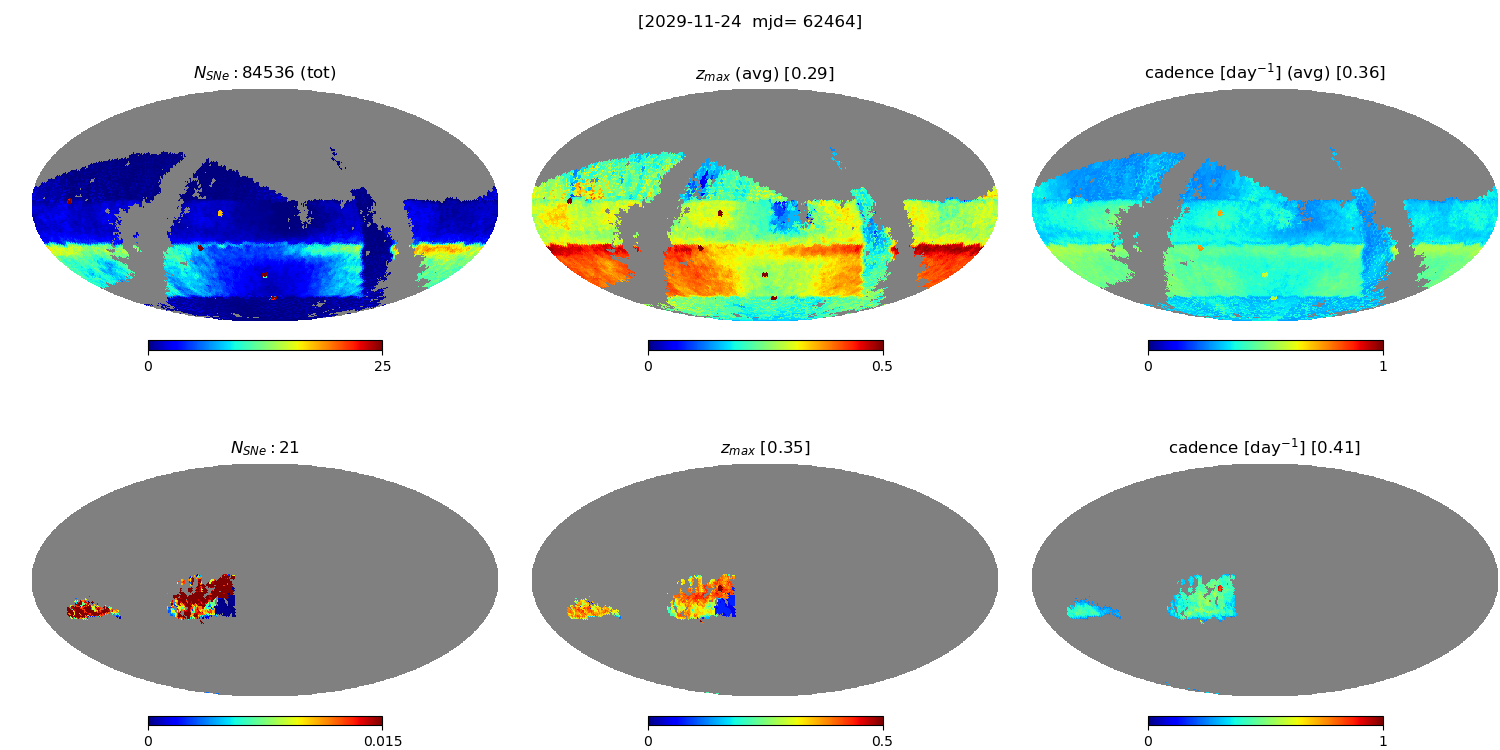
\includegraphics[width=\linewidth]{nsn/mothra_2045_02611.png}
      \caption{Example of cadence analysis maps.  Cadence {\em
          Mothra\_2045}, mjd=62464 (2029-11-24) {\em Upper panels:}
        (left) total number of well sampled supernovae per healpixel,
        (middle): median \zmed after 2611 days of survey, (right):
        median cadence, after 2611 days of survey. {\em Lower panels:}
        (left) number of SNe~Ia peaking at mjd=62464 and passing the
        light curve quality cuts (middle) \zmed, i.e.  maximum
        redshift at which a SN peaking at mjd=62464 would pass the
        requirements}
    \end{center}
\end{sidewaysfigure}

\myparagraph{Results}

We have conducted the analysis described above on all the cadences released
so far.  The final maps that report, for each healpixel (1) the final
number of SNe (2) the mean redshift limit
($\left<z_{\mathrm{faint|med}}\right>$) reached (3) the average
(restframe) cadence obtained are included in appendix
\ref{sec:wfd_maps} (figures \ref{fig:altsched_rolling_good_weather} to
\ref{fig:feature_baseline}). Finally, the animations that show the evolution
of the maps as the survey unfolds are available at the following address:
\begin{center}
  \href{http://supernovae.in2p3.fr/~nrl/lsst_sn_cadence}{http://supernovae.in2p3.fr/\~{}nrl/lsst\_sn\_cadence}
\end{center}
Inspecting these maps, we essentially recover the ranking of cadences
presented in the previous section.  We note that on some cadences,
especially the rolling cadences, the average properties (size and
depth) of the SN sample vary significantly as a function of the sky
direction. Some of these effects are related to seasonality (better
seeing allows to go deeper, for example) and depend on how realistic
the \opsim weather and seeing logs are. Others are clearly artefacts
of the observing cadence and can be corrected. For example, the on the
{\tt Mothra} and {\tt SLAIR} rolling cadences, are lines clearly
visible which correspond to depleted regions at the boundary between
the areas observed each year. The same is true on altsched rolling,
which also displays a strongly depleted region, at the region where
the scheduler switches between the upper and lower declination area.
Cures exists for these effects and are being discussed. 

Our primary metrics, ($z_{\mathrm{faint|median}}$, $N_{\mathrm{faint|median}}$) 
presented in section \ref{sec:metrics}, can be derived from these
maps.  Figures \ref{fig:nsn_zmax_med} and \ref{fig:nsn_zmax_faint}
give a synthetic presentation of our cadence evaluation, in the planes
(\zfaint, \nsnfaint) and (\zmed, \nsnmed), respectively.

\begin{sidewaysfigure}
  \begin{center}
    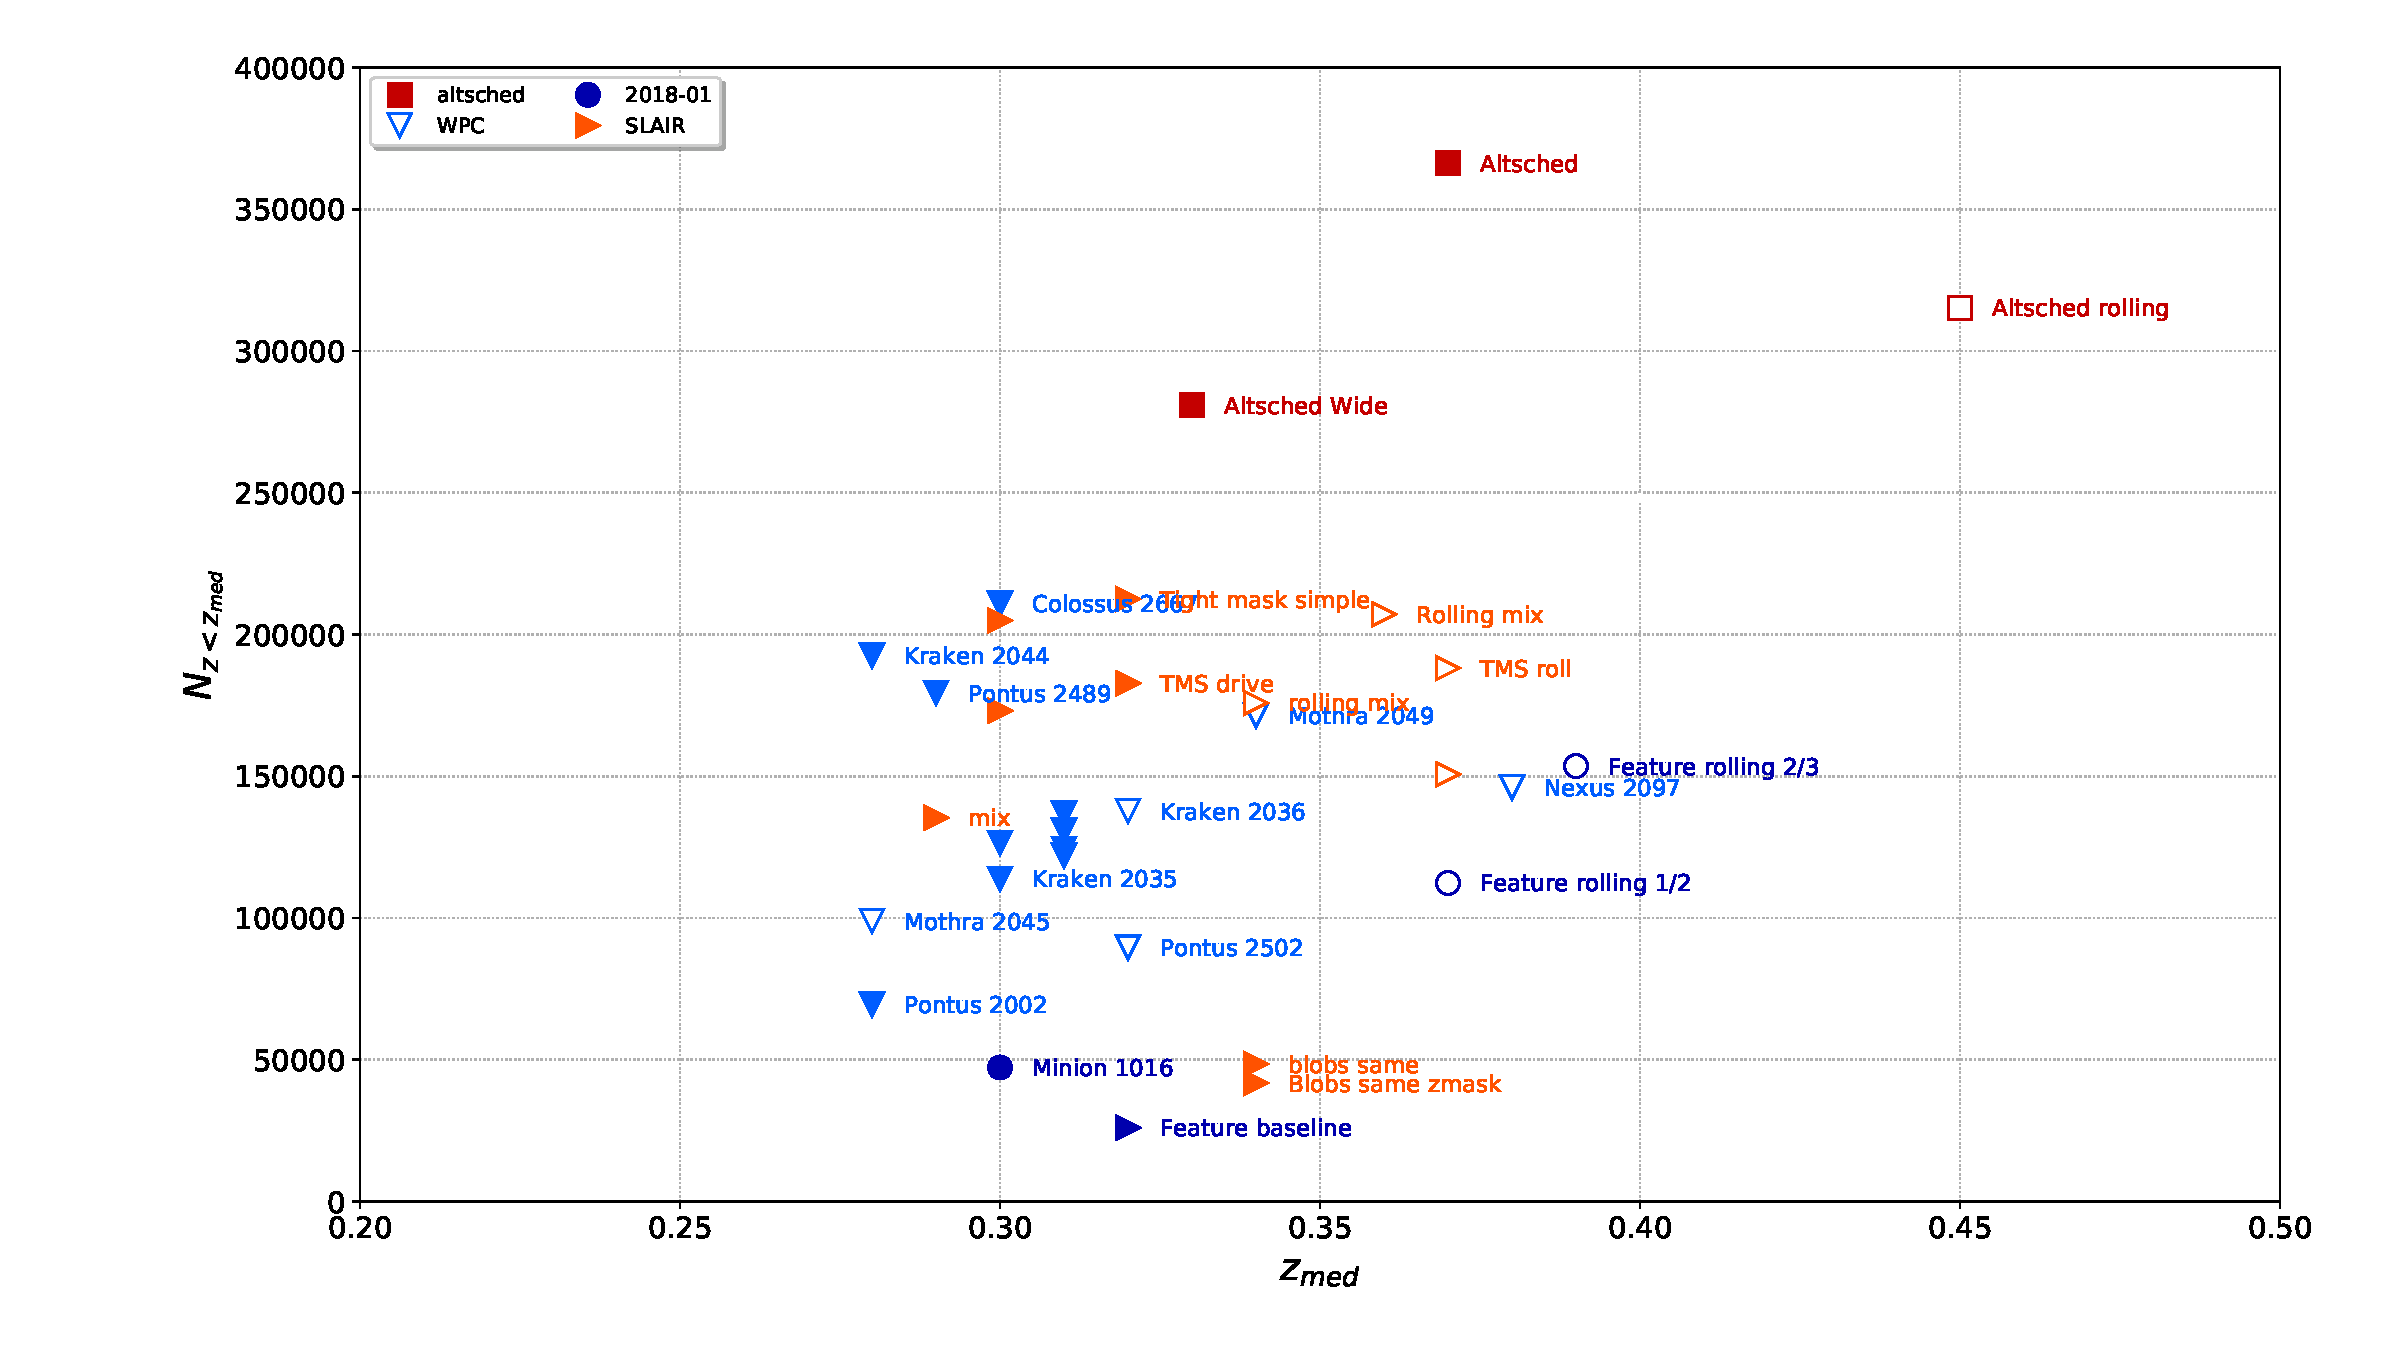
\includegraphics[width=\linewidth]{nsn/summary_plot_wfd_mediansn.pdf}
    \caption{Representation of the cadences analyzed in this study in
      the plane (\zmed, \nsnmed). This gives an assessement, for each
      cadence, of (1) the sample depth, i.e. at which redshift the
      median SN no longer passes the requirements listed in section
      \ref{sec:sn_sampling_requirements} and (2) the size of the
      subset of well-sampled SNe~Ia.}
    \label{fig:nsn_zmax_med}
  \end{center}
\end{sidewaysfigure}

\begin{sidewaysfigure}
  \begin{center}
    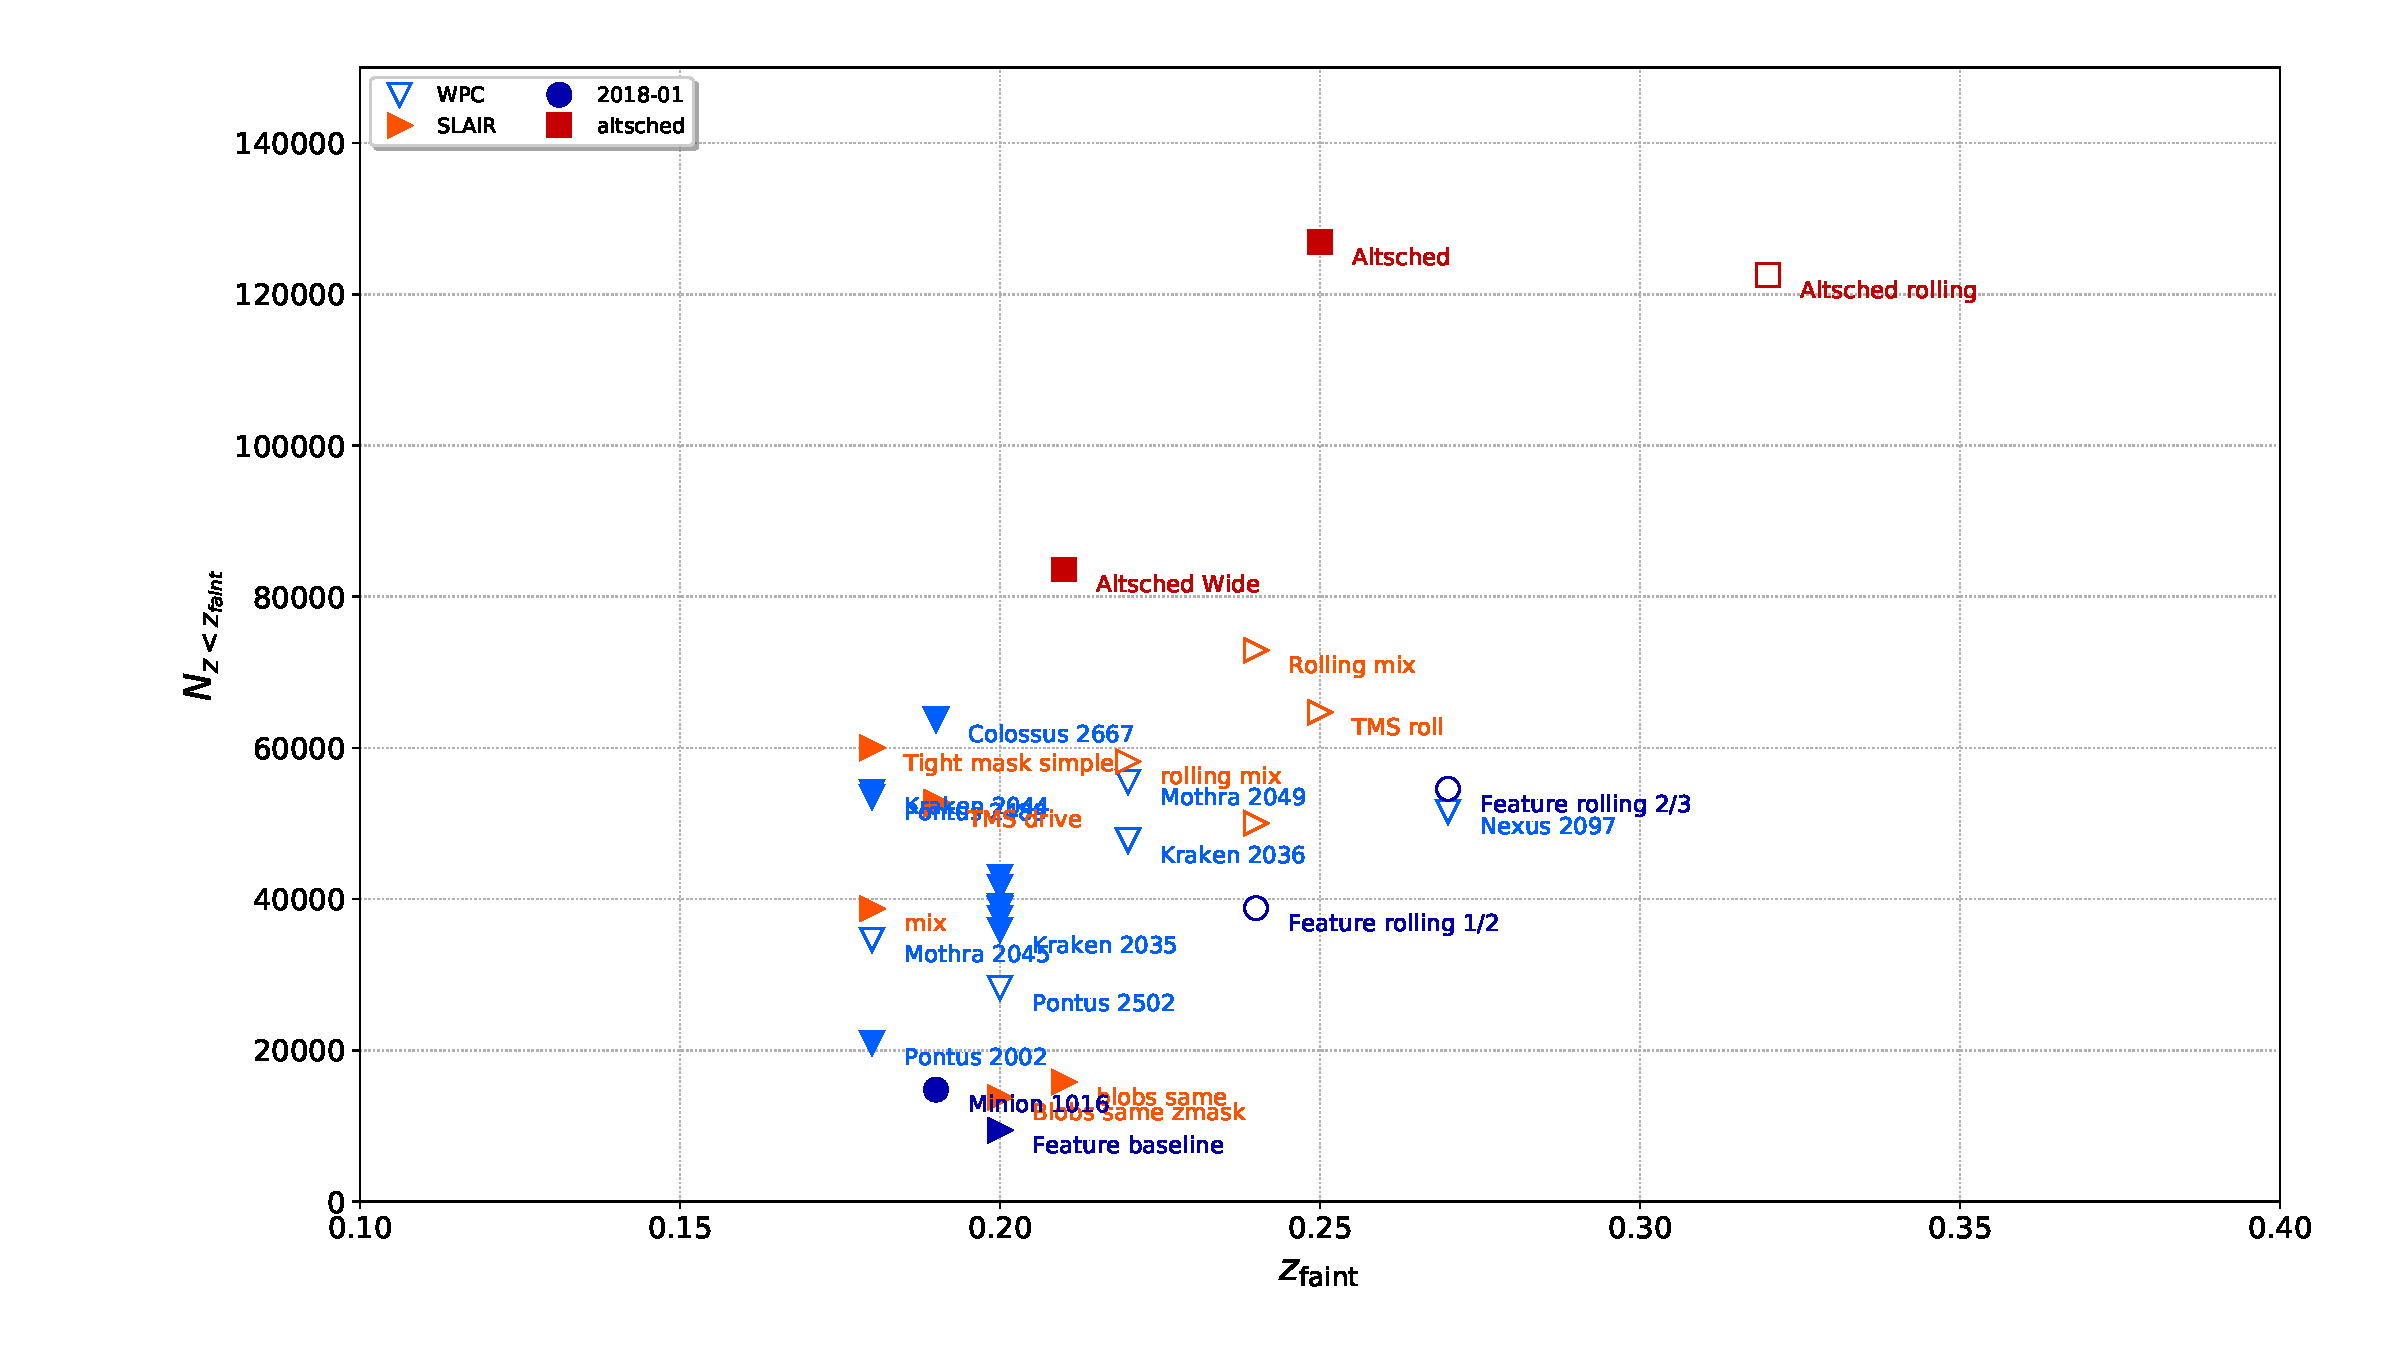
\includegraphics[width=\linewidth]{nsn/summary_plot_wfd_faintsn.pdf}
    \caption{Representation of the cadences analyzed in this study in
      the plane (\zfaint, \nsnfaint). This gives an assessement, for
      each cadence, of (1) the redshift limit of the survey, i.e. at
      which redshift the faintest SN no longer passes the requirements
      listed in section \ref{sec:sn_sampling_requirements} and (2) the
      size of the redshift limited SN~Ia sample produced by LSST.}
    \label{fig:nsn_zmax_faint}
  \end{center}
\end{sidewaysfigure}

Again, we recover our previous ranking.  The rolling version of
\altsched is the best performing cadence.  It will allow us to build a
very deep sample \zmed $\sim 0.45$ of more than well sampled 300,000
SNe.  {\tt altsched} covers more area, at the expense of a lower
cadence.  As a consequence, it is not as deep, but allows to obtain a
larger number of well-sampled SNe.

Most of the cadences released for the white paper call do not allow to
go as deep, no to secure as many well sampled SNe. The best \opsim and
\slair rolling cadences allow to reach redshift limits that are
similar to the non-rolling version of \altsched and yield samples that
are about 40\% smaller. All of them, in particular {\tt rolling mix}
and {\tt tms roll} implement the design principles exposed in section
\ref{sec:wfd_cadence_key_properties}. Why they do not reach the
performances of {\tt altsched rolling} is unclear at this point and is
being investigated.


\subsection{Overlap with 4MOST extragalactic surveys}

\myparagraph{Method}

The 4MOST facility will be a highly multiplexed, optical, fibre-fed
spectrograph mounted on the 4-metre VISTA telescope. It is due to
start operations at the end of 2022. Its wide field of view (4.1 sq
deg), high multiplex (1600 fibres feeding low-resolution spectrographs
suitable for extragalactic science plus $\sim 800$ fibres feeding a
high-resolution spectrograph, primarily for galactic science) and
geographical location (near the Paranal site in Chile) makes 4MOST an
ideal spectroscopic follow-up facility for 4MOST. The scientific
synergy potentially covers a very wide variety of science goals. Here
we focus on the synergy for follow-up of transients and varying
sources.

The 4MOST-TiDES survey plans to piggy-back on other 4MOST
extragalactic surveys, and will use a small subset of the fibres in
each pointing to observe live transients and the host galaxies of
previously-discovered transients. The 4MOST extragalactic surveys will
be carried out over a large fraction of the southern sky, shown in
Figure~\ref{4most_sky}.  There is also a component of TiDES that aims
to obtain spectral time-sequences of AGN in 4MOST's deep fields (that
are likely to coincide with at least a subset of LSST's deep fields,
TBD), for reverberation mapping.

\begin{figure}[!htbp]
\begin{center}
  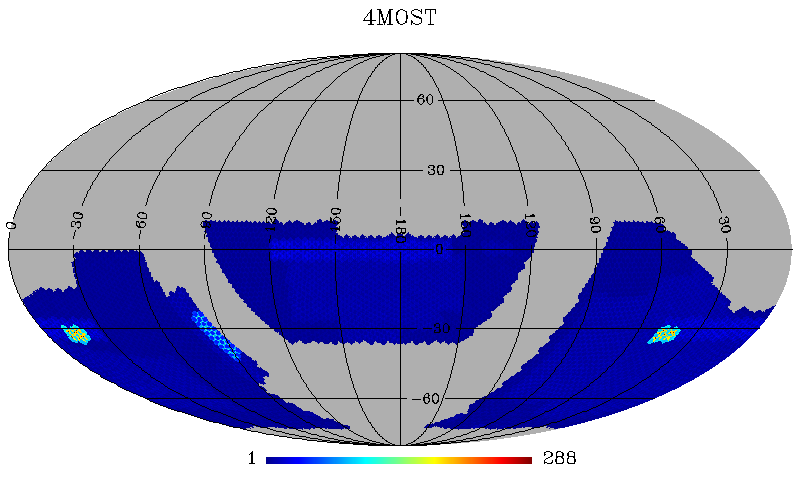
\includegraphics[width=10.0cm]{overlap_4MOST/4most_fndep.png}
\end{center}

\caption{One realisation of the sky coverage of 4MOST extragalactic
  surveys, colour coded by number of visits. This is based on
  4MOST-4FS survey simulation round9/c/run01 dated 2018-5-14. Note
  that the 4MOST survey design is still in progress and the map is
  likely to change.}
\label{4most_sky}
\end{figure}

There is a preference for 4MOST to observe within the approximate
declination range seen in Figure~\ref{4most_sky} for several
reasons. One is not to duplicate other facilities in the North (such
as DESI, Subaru-PFS and WEAVE). Another is that the winds from the
north at Paranal can make it difficult to observe in that
direction. Similarly, 4MOST prefers not to observe far South because
of inefficiency when observing at high airmass. The 4MOST Atmospheric
Dispersion Compensator works optimally upto zenith distances of 55
degrees, equivalent to airmass of $\sim1.75$. At larger airmasses,
light is lost at the ends of the spectrum. Because VISTA is at
latitude $\sim -24.7$ degrees, one can therefore observe theoretically
to declination of $\sim -80$ degrees at the meridian. In practice
4MOST will not go much below declination of $-70$ degrees, except in
the Magellanic Clouds, as observations get much harder to schedule if
one wants to stay beyond airmass $\sim 1.75$ for an hour. However,
there could be exceptions if, for example, there was an interesting
deep field a bit north or south of the current range.

In addition to the extragalactic surveys, 4MOST will survey the Milky
Way disk area with the same 1600 fibres feeding low-resoution + 800
fibres feeding high resolution spectrographs, but this will be mainly
in bright time and geared toward brighter targets and hence less
suitable for extra-galactic follow-up. However, this survey might be
interesting for follow-up of stellar variables.

Finally, we note that a Call for Letters of Intent for 4MOST community
observations is expected to be opened next summer (2019).


\myparagraph{Results}

In order to compare the overall spatial coverage of 4MOST and the
various possible LSST survey strategies, we have divided the sky into
healpixels with NSIDE=256 (approx. 0.052 sq deg resolution). We are
considering only the WFD components of the LSST survey strategies
here.
For the LSST surveys we used each OpSim simulation (with a dither
pattern superimposed that gives a high spatial uniformity of depth) to
make a healpix map, and kept all healpixels with more than 500 visits
over 10 years.

\begin{comment}
\footnote{The code used to
  make these is the script
  {\tt https://github.com/rbiswas4/OpSimSummary/blob/master/scripts/make\_simlibs.py}}
\end{comment}

For 4MOST, we used the most recent 4MOST 4FS simulation,
(round9/c/run01 dated 2018-5-14) and made a Healpix map using the
central coordinates of each 4MOST tile, and assuming a hexagonal field
of view with area 4.1 sq deg. Each Healpixel with one or more visits
was kept.
 
We then calculated number of overlapping healpixels and multiplied by the
spatial area of one healpixel to give the overlapping areas shown in
Table~\ref{4most_overlap_tab}. Maps are shown in Figures~\ref{overlap_maps} - \ref{overlap_maps_c}.

\begin{table}[!htbp]
  \begin{center}
 \caption{Overlapping areas between LSST WFD and 4MOST extragalactic surveys}
\begin{tabular}{cc}\hline \hline
  LSST OpSim run & Overlapping area (sq deg) \cr\hline \hline
  mothra\_2045   &	11702 \cr
  colossus\_2667 &	12644 \cr
kraken\_2026   &	12644 \cr
kraken\_2036   &        12644 \cr
pontus\_2489   &	12644 \cr  
pontus\_2502   &	12644 \cr
colossus\_2664 &        12805 \cr
colossus\_2665 &	13096 \cr
pontus\_2002   &	15000 \cr
  \hline
\end{tabular}
\end{center}
\label{4most_overlap_tab}
\end{table}




\subparagraph{Temporal overlap}

4MOST will typically visit each part of the sky twice, for about one
hour exposure ($3\times$ 20 mins) exposures each time (but we
emphasise again that the details of the 4MOST survey are still under
discussion). Clearly, for follow-up of live transients it is important
that 4MOST observes in the areas of sky the LSST has visited recently
(within the lifetime of the transients concerned). For example if LSST
follows a rolling cadence then to maximise trabnsient science, 4MOST
should observe in the same declination range.  Coordination of LSST
and 4MOST surveys is essential.


\myparagraph{Conclusion}

Of the LSST cadence simulations considered, pontus\_2002 gives the
largest overall spatial overlap, of approx. 15,000 sq deg, compared to
approximately 12,000-13,000 sq deg for the other surveys. The extended
declination range of pontus\_2002 increases the overlap with 4MOST,
but goes a little too far in that some of extended LSST area is then
not covered by 4MOST.

As stressed above, temporal coordination of the 4MOST and LSST surveys is
essential if transient science is to be maximised.


\subsection{Peculiar velocity}

\myparagraph{Method}

Peculiar velocities provide a measure of $f\sigma_8$, which in turn probes gravity.  As precise distance indicators Type~Ia supernovae (SNe~Ia)
can provide precise peculiar velocities of their host galaxies \citep{2006PhRvD..73l3526H,2011ApJ...741...67D}.

\citet{2017ApJ...847..128H} calculated the  expected precision of $f\sigma_8$ using LSST-discovered SNe~Ia.
The Fisher information matrix of a random Gaussian field with mean zero and covariance $C(k)$ parameterized by $\lambda$ is
\begin{equation}
F_{ij} = \frac{V}{2}\int \frac{d^3k}{(2\pi)^3} \text{Tr}\left[ C^{-1} \frac{\partial C}{\partial \lambda_i} C^{-1}
\frac{\partial C}{\partial \lambda_j} \right].
\end{equation}
The covariance
\begin{equation}
C = P_{vv}(k) + \frac{\sigma^2}{n}
\end{equation}
has contributions from the power spectrum, noise in the velocity measurement, and the density of velocity probes.
In the sample variance limit for a sample with fixed depth, the variance in $f\sigma_8$ (and other $\lambda$ parameters)
is thus inversely proportional to the survey solid-angle $\Omega$, whereas
in the shot-noise limit the variance is inversely proportional to $\Omega n^2 \propto N^2/\Omega$, where $n$ is the number density,
and $N$ is the total number of supernovae.  


\myparagraph{Results}
N.~Regnault kindly provided us with his assessment of the number and solid-angle of $z<0.2$ supernova pre-maximum discoveries 
for the survey candidates provided by the Project.  Based on these numbers we calculate the Figures of Merit in the two regimes 
(normalized with respect to the average of all the surveys),
with our results shown in 
Table~\ref{table:ref}.  The results of \citet{2017ApJ...847..128H}  indicate that after 10 years,
LSST supernovae are at neither extreme; we thus adopt the average of the two FoM's as what we advocate for the survey.


\begin{table}
\caption{SN~Ia Figures of Merit of Project survey candidates
in  the shot-noise and the survey-variance limits.  The final column is the average
of the two Figures of the Merit.\label{table:ref}}
\centering
\begin{tabular}{crrr}
  \hline
  \hline
Survey & FoM (shot) & FoM (survey) & FoM (avg)\\
\hline
\hline
feature\_baseline\_10yrs & 0.025 & 0.642 & 0.334  \\
blobs\_same\_zmask10yrs & 0.048 & 0.859 & 0.453  \\
blobs\_same\_10yrs & 0.064 & 0.859 & 0.462  \\
feature\_rolling\_half\_mask\_10yrs & 0.175 & 0.987 & 0.581  \\
minion\_1016 & 0.093 & 1.109 & 0.601  \\
pontus\_2502 & 0.132 & 1.107 & 0.62  \\
feature\_rolling\_twoThird\_10yrs & 0.187 & 1.104 & 0.645  \\
mothra\_2045 & 0.226 & 1.134 & 0.68  \\
pontus\_2002 & 0.224 & 1.157 & 0.691  \\
rolling\_10yrs & 0.581 & 0.838 & 0.709  \\
nexus\_2097 & 0.28 & 1.166 & 0.723  \\
kraken\_2035 & 0.705 & 0.823 & 0.764  \\
tms\_roll\_10yrs & 0.424 & 1.119 & 0.771  \\
kraken\_2036 & 0.437 & 1.141 & 0.789  \\
baseline2018a & 0.779 & 0.834 & 0.807  \\
kraken\_2042 & 0.794 & 0.858 & 0.826  \\
colossus\_2665 & 0.797 & 0.861 & 0.829  \\
colossus\_2664 & 0.814 & 0.884 & 0.849  \\
alt\_sched\_rolling & 0.804 & 0.92 & 0.862  \\
altsched\_rolling\_good\_weather & 0.815 & 0.92 & 0.868  \\
tight\_mask\_simple\_10yrs & 0.6 & 1.141 & 0.871  \\
kraken\_2026 & 0.947 & 0.838 & 0.892  \\
tight\_mask\_10yrs & 0.646 & 1.155 & 0.901  \\
mothra\_2049 & 0.671 & 1.161 & 0.916  \\
rolling\_mix\_75\_10yrs & 0.85 & 1.007 & 0.928  \\
tms\_drive\_10yrs & 0.806 & 1.09 & 0.948  \\
rolling\_mix\_10yrs & 0.958 & 1.011 & 0.984  \\
cadence\_mix\_10yrs & 1.012 & 1.012 & 1.012  \\
blobs\_mix\_zmask10yrs & 1.432 & 1.008 & 1.22  \\
pontus\_2489 & 2.052 & 0.97 & 1.511  \\
colossus\_2667 & 2.365 & 1.004 & 1.684  \\
alt\_sched & 2.788 & 0.91 & 1.849  \\
kraken\_2044 & 2.565 & 1.162 & 1.863  \\
alt\_sched\_twi & 2.816 & 0.927 & 1.871  \\
altsched\_18\_\_90\_30 & 2.581 & 1.187 & 1.884  \\
altsched\_18\_\_90\_40 & 2.594 & 1.187 & 1.89  \\
altsched\_good\_weather & 2.914 & 0.91 & 1.912  \\
\hline
\end{tabular}
\end{table}

\begin{comment}
rolling\_10yrs  & 0.581 & 0.838 & 0.709  \\
mothra\_2045  & 0.226 & 1.134 & 0.680  \\
blobs\_same\_zmask10yrs  & 0.048 & 0.859 & 0.453  \\
rolling\_mix\_75\_10yrs  & 0.850 & 1.007 & 0.928  \\
alt\_sched\_twi  & 2.816 & 0.927 & 1.871  \\
alt\_sched\_rolling  & 0.804 & 0.920 & 0.862  \\
pontus\_2489  & 2.052 & 0.970 & 1.511  \\
kraken\_2044  & 2.565 & 1.162 & 1.863  \\
pontus\_2002  & 0.224 & 1.157 & 0.691  \\
tms\_drive\_10yrs  & 0.806 & 1.090 & 0.948  \\
tight\_mask\_simple\_10yrs  & 0.600 & 1.141 & 0.871  \\
baseline2018a  & 0.779 & 0.834 & 0.807  \\
altsched\_18\_\_90\_40  & 2.594 & 1.187 & 1.890  \\
kraken\_2026  & 0.947 & 0.838 & 0.892  \\
feature\_baseline\_10yrs  & 0.025 & 0.642 & 0.334  \\
blobs\_same\_10yrs  & 0.064 & 0.859 & 0.462  \\
cadence\_mix\_10yrs  & 1.012 & 1.012 & 1.012  \\
feature\_rolling\_half\_mask\_10yrs  & 0.175 & 0.987 & 0.581  \\
pontus\_2502  & 0.132 & 1.107 & 0.620  \\
colossus\_2667  & 2.365 & 1.004 & 1.684  \\
kraken\_2036  & 0.437 & 1.141 & 0.789  \\
tms\_roll\_10yrs  & 0.424 & 1.119 & 0.771  \\
rolling\_mix\_10yrs  & 0.958 & 1.011 & 0.984  \\
altsched\_rolling\_good\_weather  & 0.815 & 0.920 & 0.868  \\
altsched\_18\_\_90\_30  & 2.581 & 1.187 & 1.884  \\
tight\_mask\_10yrs  & 0.646 & 1.155 & 0.901  \\
alt\_sched  & 2.788 & 0.910 & 1.849  \\
colossus\_2665  & 0.797 & 0.861 & 0.829  \\
colossus\_2664  & 0.814 & 0.884 & 0.849  \\
mothra\_2049  & 0.671 & 1.161 & 0.916  \\
kraken\_2042  & 0.794 & 0.858 & 0.826  \\
minion\_1016  & 0.093 & 1.109 & 0.601  \\
kraken\_2035  & 0.705 & 0.823 & 0.764  \\
nexus\_2097  & 0.280 & 1.166 & 0.723  \\
blobs\_mix\_zmask10yrs  & 1.432 & 1.008 & 1.220  \\
feature\_rolling\_twoThird\_10yrs  & 0.187 & 1.104 & 0.645  \\
altsched\_good\_weather  & 2.914 & 0.910 & 1.912  \\
\end{comment}

\myparagraph{Conclusion}

We are in the course of refining the Figure or Merit, taking into account survey geometry, combining both survey variance and shot noise.
Any significant changes in our findings will lead to an update of our relative
ranking of the surveys.








\subsection{Photometric classification}

\myparagraph{Method}
The aim of this investigation is to analyse the affect a particular cadence has
on ones ability to photometrically classify supernova. This investigation has been carried out by the
developers of {\sc snmachine} who work in the Supernova Working Group under the umbrella of the Dark Energy Science
Collaboration (DESC). {\sc snmachine} is a DESC product that is used as a photometric
classification pipeline \cite{lochner2016photometric}.

The motivation for this work comes from the desire to identify as many Supernova
as Type 1a in order to help constrain the nature of Dark Energy.
LSST will observe many more Supernova than ever before, but at a rate that is
not feasible for all of these transients to be spectroscopically followed up and
confirmed as Type 1a or not.
Thus, the ability to classify these objects photometrically will be very
important. If one can obtain a greater set of Type 1a's, an updated Hubble
digram plot can be produced and the fundamental parameters of the cosmological
model can be tested further.

In order to conduct this analysis, use of third
party software, {\sc SNANA}, has been used to generate light curves that correspond to
different cadences runs from {\sc OpSim} outputs. The generated light curves are
then used as inputs in the {\sc snmachine} pipeline, an example of which is
shown below.

An interpolation is done for the between the sampled points to produce a smooth
light curves with one can then apply a wavelet decomposition to. The resulting
wavelet coefficients are then processed further to reduce dimensionality using a
principle component analysis. These principle components are what are then
provided as features to a random forest classifier. To ensure a controlled test,
for each cadence run a classifier is trained on 2000 light
curves only and then tested on the remaining set of light curves that are in the
corresponding dataset produced from {\sc SNANA} in relation to specific {\sc OpSim} cadence
simulation. 

\myparagraph{Results}
The results for which are shown below in Figure\ref{fig:rocs}
\begin{figure}
  \centering
  \subfigure[DDFY1]{\label{fig:ddfy1}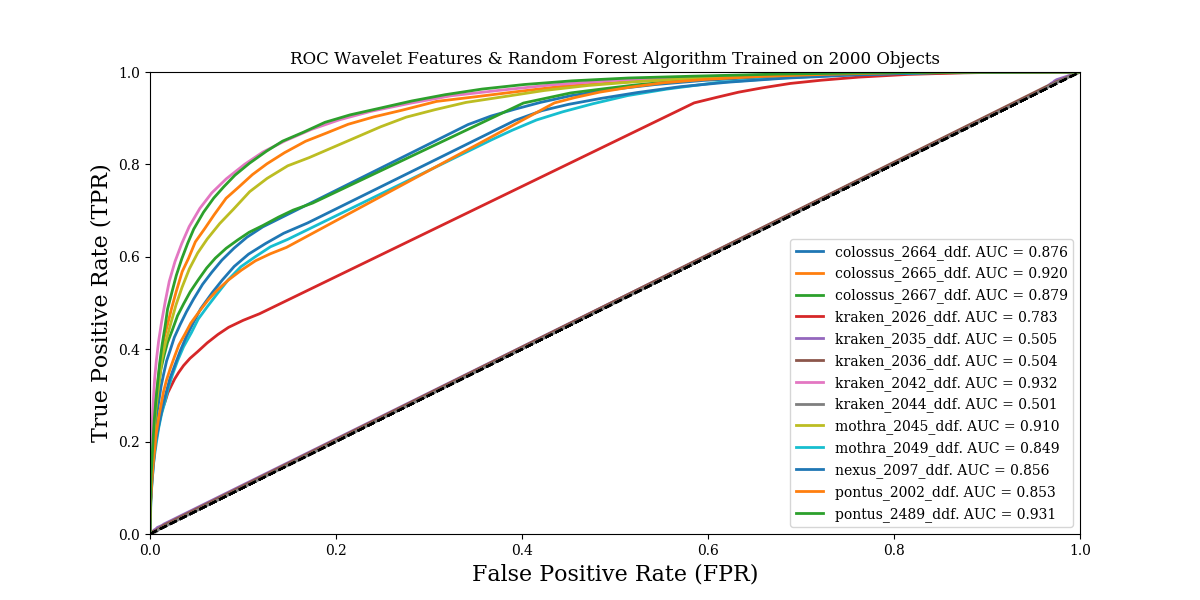
\includegraphics[width=0.8\textwidth]{classification/photometric_classification_roc_results_ddfY1.png}}
    \subfigure[DDFY10]{\label{fig:ddfy10}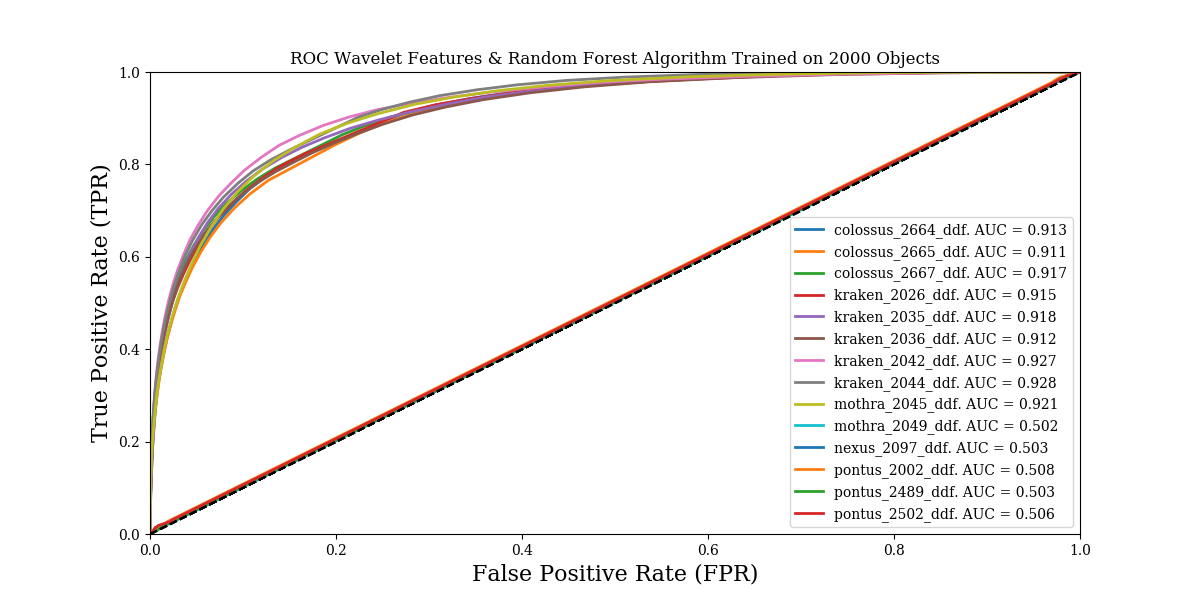
\includegraphics[width=0.8\textwidth]{classification/photometric_classification_roc_results_ddfY10.png}}
   \caption{Comparison for the DDFY1 and DDFY10 ROC curves}\label{fig:rocs}
\end{figure}

Figure\ref{fig:ddfy1} shows the
comparative classification performances between 13 cadences for the Deep
Drilling Fields of Year 1 whereas Figure\ref{fig:ddfy10} compares the same
cadences for the Deep Drilling Fields over the entire survey.

The area under the Receiver Operating Characteristic (auROC) curves were chosen as the metric
to evaluate the performance. It was felt this single scalar would be most useful
for being able to differentiate the ability of the various cadence strategies
to perform photometric classification.

By interpolating the sampled light curved with Gaussian process and then applying a
wavelet decomposition to these interpolated light curves, one obtains features
that can be provided to a classifier, in this case a Random Forest algorithm.
The performance of the interpolation is directly affected by the amount of
samples one has on the light curve. More samples improves the reliability of the
Gaussian processes and thus provided better features through via the wave decomposition.

Therefore it can be understood that in order to classify transients, short sampling of a light
curve is important. This is particularly important for early classification
leading to possible spectroscopic follow up. Work from Philippe Gris
investigates
the number of \emph{well-sampled} light curves one can obtain from the different
cadence strategies. Separate to that study, analysis of cadence impact on
classification is done here, but nonetheless, a well sampled light curve would
indeed boost classification rate. Thus, before any analysis is conducted, one
could assume a rolling cadence with 2 to 3 days would be beneficial to the
cause.
With this in mind, the results of the analysis shown here do not in particular
point to a specific cadence as be favourable, but the performance of some
strategies do not perform as well as others in the Year 1 case and over the
Year 10 full survey.

This research can be taken further in several ways and there are plans to
continue this analysis for Wide-Fast-Deep cadence runs also. Work is currently
taking place to investigate the performance of classifiers trained on DDF runs
and then tested on WFD. Work is also being carried out for a comparative stufy
of WFD cadence runs much like what has been shown above for DDFY1 and DDFY10.
Further to the two DDF runs presented, further analysis will be carried out for
more years to see the performances for years in between and to see if there
are classification trends that change through the lifetime of the survey. It is
also hoped that number of Supernova used for training affects classification
performances, this work is done but alternations are required to the code for a complete
analysis. Finally it would be beneficial to understand the elements of each cadence
strategy to give further insight as to why certain cadences perform the way they do.

\myparagraph{Conclusions} 
It is difficult to say at this stage which cadence is preferred until further
analysis is done, and one leaves this to the working group leaders to draw
concrete conclusions.


\subsection{$w_0~w_a$ constraints}

\myparagraph{Method}

In order to assess the impact of the cadence on the cosmological analysis possible with supernovae, we compute the Dark Energy Task force figure of merit \cite{2006astro.ph..9591A} in the dark energy parameters $w_0-w_a,$ for a few scenarios. The supernova sample is simulated using (\strech, \sncolor) distributions estimated from \cite{2016ApJ...822L..35S} (High-z G10 parameters) and production rates from  \cite{2008ApJ...682..262D}.

In the first instance, the supernova sample is simulated following roughly the same prescription as that outlined in the recent Science Requirements Document \cite{2018arXiv180901669T}, with small changes to the host redshift selection. For the SRD we adjusted the survey size simulated to ensure roughly 112 000 SNe after host selection cuts from a 4MOST-like ground based telescope. This is the largest determinant of the final size, and so in order to test for differences in the survey strategy we initially doubled the survey size simulated, and then tested a few cadences without requiring any spectrosopic host redshift. This was to ensure that the host-$z$ follow up was not the most important characteristic.
In addition, we imposed a more restrictive cut on the fitted colour in the SAL2T fit from $\sigma(c) < 0.08$ to $\sigma(c) < 0.05.$ Insodoing we are forcing that the supernovae that survive are of higher quality than in the DESC SRD.

In order to test more strongly the impact of the wide field cadence on the overall cosmology, we ran simulations including \textit{only the WFD survey} in addition to a low-$z$ (e.g. Foundation-like) data set. We compared the cosmology results from the WFD+Foundation surveys for the {\tt kraken\_2026, kraken\_2035} and {\tt altsched, altsched\_rolling} cadences. Finally we show the results with and without spectroscopic host redshift selection for the baseline {\tt kraken\_2026} survey.

We have included only statistical errors: for speed of computation we have neglected the astrophysical systematics. This will be relaxed in future versions.


\begin{figure}
  \begin{center}
  \subfigure[w0-wa ellipses]{\label{fig:w0wa}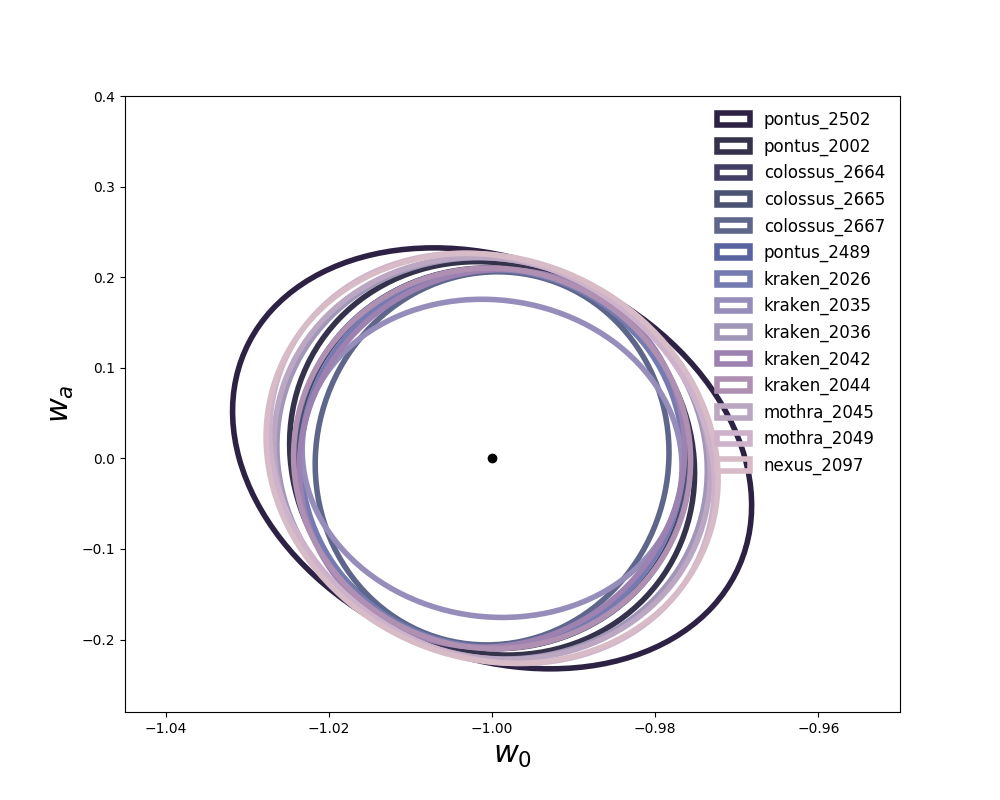
\includegraphics[width=0.7\textwidth]{w0wa/FM_plot_cadence_updated.png}}
    \subfigure[FoM vs observing strategy]{\label{fig:snfom}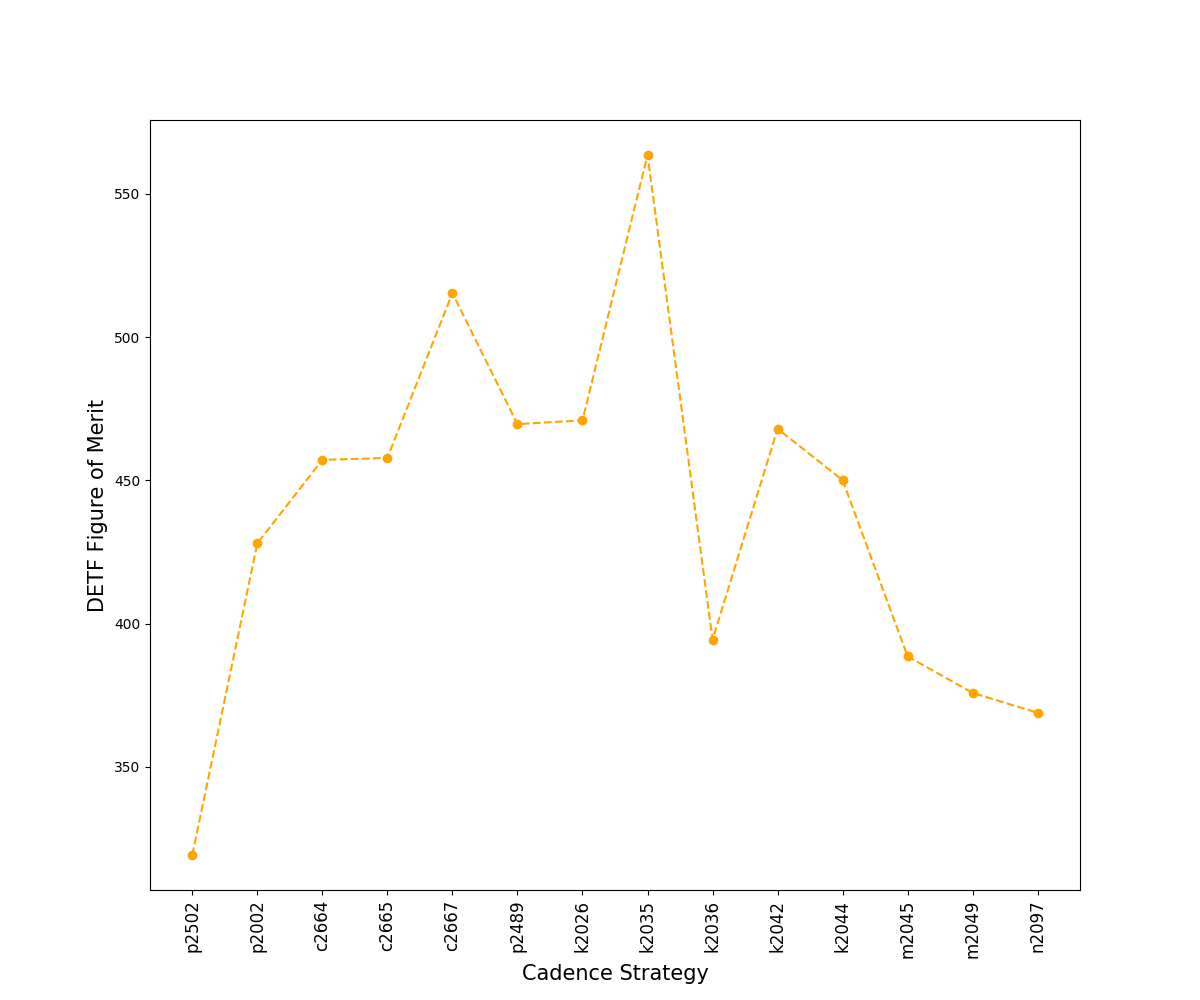
\includegraphics[width=0.7\textwidth]{w0wa/FoM_cadence_updated.png}}
    \caption{Cosmology constraints across cadence types: the ellipses in the $w_0-w_a$ plane (a) and the dark energy figure of merit is shown (b) are shown. }
    \end{center}
\end{figure}
\myparagraph{Results}
The largest difference in the Figure of Merit (Fig. \ref{fig:w0wa}) we find is a factor of two between the highest FoM (kraken\_2035) and the lowest FoM (pontus\_2502) if both WDF and DDF surveys are taken into account. The lowest-performing strategy has two alternating bands in declination, switching in alternate years, which is expect to perform poorly. The fact kraken\_2035 is performing better compared to other observing strategies may be explained by the higher number of DD fields observed (9 whereas all other strategies considered 5 fields).

\altsched~ and kraken\_2026 show highest FoMs in WFD-only scenarios (Fig. \ref{fig:snfom}) followed by rolling\_mix, kraken\_2035 , \altsched\_rolling and rolling observing strategies. One may observe that these cadences exhibit the highest FoMs as the following classification shows:
\begin{itemize}
\item{500 $\leq$ FoM}: kraken\_2035, \altsched, kraken\_226, rolling\_mix, kraken\_2035 , \altsched\_rolling and rolling ;
\item{400 $\leq$ FoM $\leq$ 500}: pontus\_2489, kraken\_2042, colossus\_2665, colossus\_2664, kraken\_2044, pontus\_2002 ;
\item{FoM $\leq$ 400}: nexus\_2049, nexus\_2097, kraken\_2026.

\end{itemize}



\myparagraph{Conclusion}





\section{Metrics and proposed observing strategies: summary}
 

\section{New proposals}

\subsection{DDF observing strategy}

In OpSim the choice to observe a given field is done on the fly according to an optimized selection function depending on criteria including (among others) observing conditions, slew time minimization, last time of visit, and total observing time. While the use of a simple metric (see below) would help in choosing another approach could be to use a pre-defined table that would specify which DDF are to be observed on a given night.

Let us consider the four reference fields \cosmos, \xmmlss, \cdfs~and \elais. Since the location are well known, it is possible to estimate when these fields are visible (that is with an altitude between 20 and 86.5 degrees) for a large enough period (typically 20 to 40 minutes) of good observing conditions (ie with airmass lower than a reference value - typically 1.5). We may define a (boolean) parameter dubbed observability equal to one when the above-mentioned conditions are filled, and 0 otherwise. This parameter is displayed on Figure \ref{fig:observability} (top). \xmmlss,\cdfs, and \elais~ are located in the same (Ra) region and may thus be observed during the same night whereas \cosmos~may be observed when all others are not visible. Season lengths of observability (Figure \ref{fig:observability} - bottom) range from 200 to 290 days.


\begin{figure}[!htbp]
\begin{center}
  
  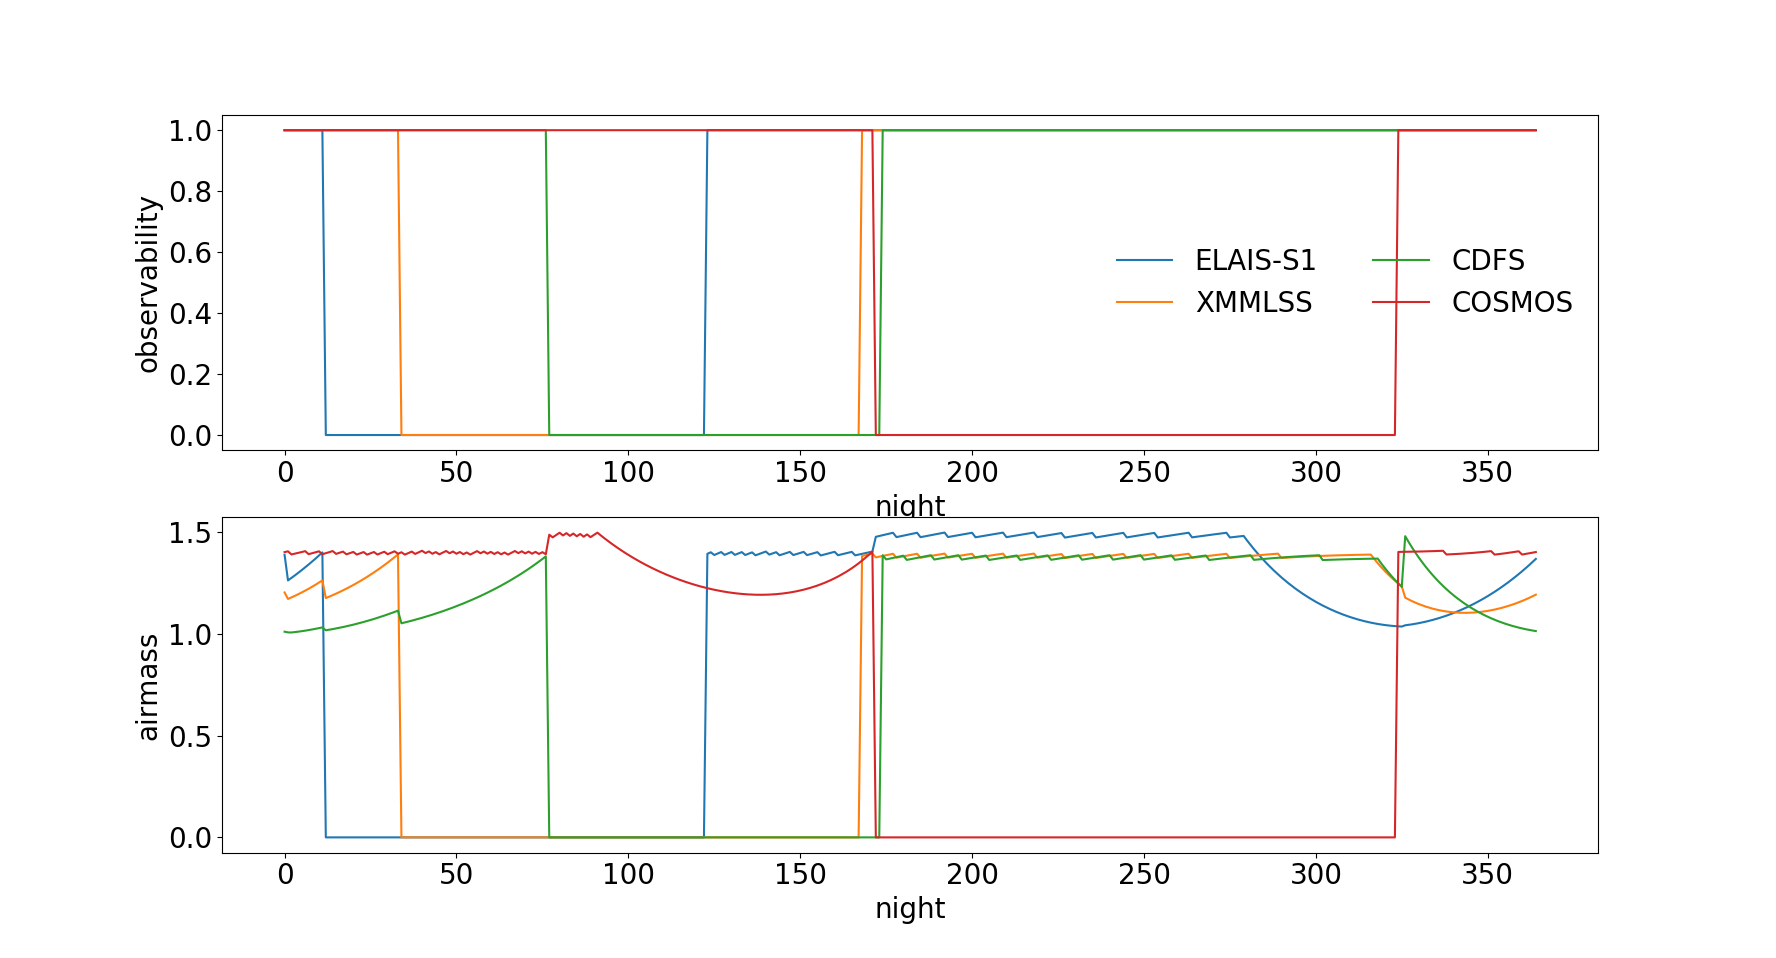
\includegraphics[width=18cm,height=12cm]{new_proposals/observability.png}
  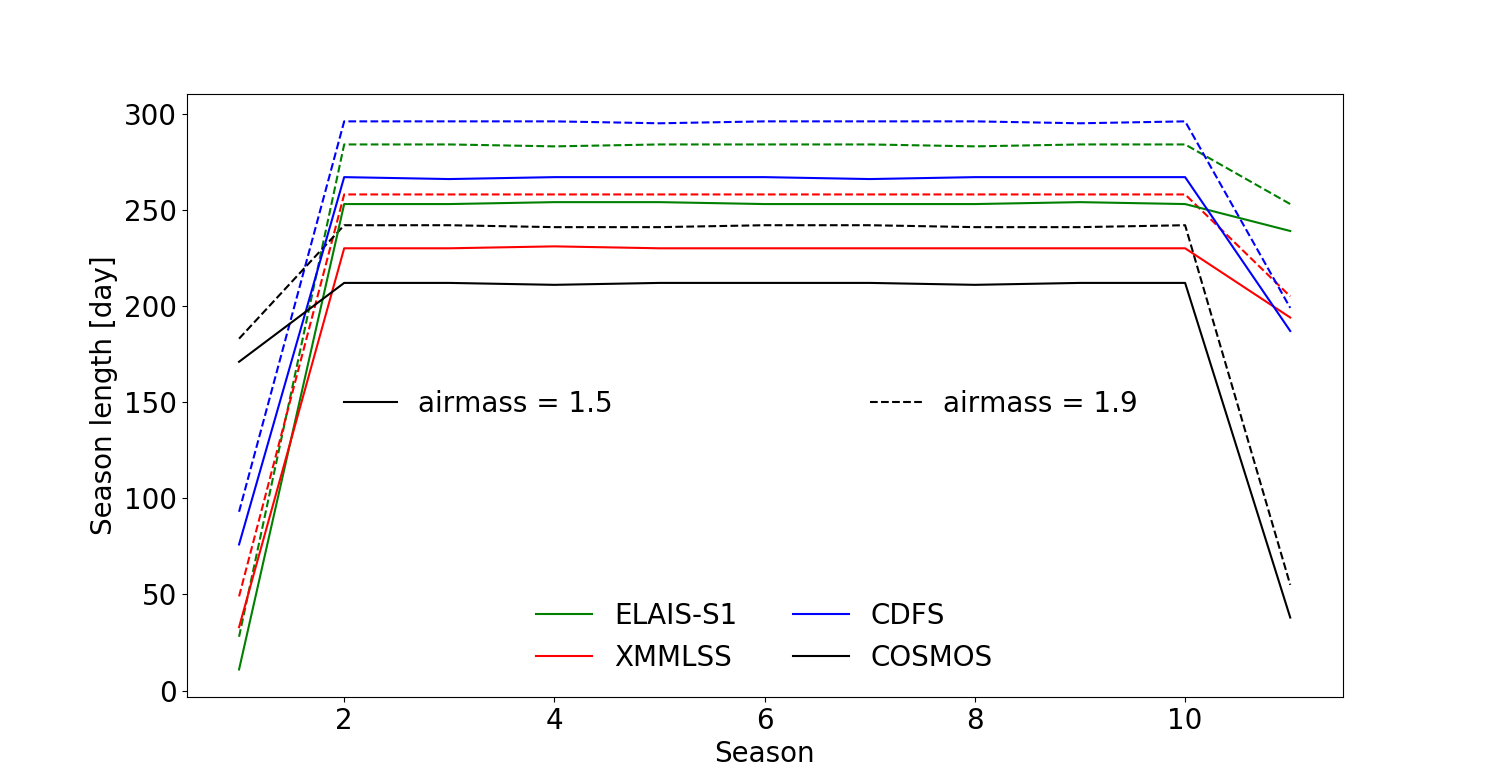
\includegraphics[width=18cm,height=8cm]{new_proposals/Season_length.png}
 \caption{Top: observability (see definition in the text) and airmass as a function of the night number (first year of LSST operation). Bottom: season length as a function of the season for an airmass limit of 1.5 (full lines) and 1.9 (dashed lines).}\label{fig:observability}
\end{center}
\end{figure}

The table of observations may be defined using median gap values \tgapcosmos~and \tgapothers~when \cosmos~and \xmmlss,\cdfs,\elais~are not observable, respectively. Observing time windows are then defined by:
\begin{itemize}
\item{[\tgapothers-w/2,\tgapothers+w/2]: \cosmos~ is observed}
\item{[\tgapcosmos-w,\tgapcosmos+w]: \xmmlss, \cdfs, \elais~are observed.}
\end{itemize}
with a width w equal to 2/3*(\tgapcosmos-\tgapothers).

\subsection{altsched rolling 80/20}

\subsection{altsched rolling 75/25}

\subsection{Adding a simple metric for SN in OpSim/SLAIR}


\section{Conclusion}

\begin{thebibliography}{9}
\expandafter\ifx\csname natexlab\endcsname\relax\def\natexlab#1{#1}\fi
\providecommand{\url}[1]{\href{#1}{#1}}
\providecommand{\dodoi}[1]{doi:~\href{http://doi.org/#1}{\nolinkurl{#1}}}
\providecommand{\doeprint}[1]{\href{http://ascl.net/#1}{\nolinkurl{http://ascl.net/#1}}}
\providecommand{\doarXiv}[1]{\href{https://arxiv.org/abs/#1}{\nolinkurl{https://arxiv.org/abs/#1}}}


\bibitem{perrett} Evolution in the Volumetric Type Ia Supernova Rate from the Supernova Legacy Survey, K.Perrett {\it et al}, The Astronomical Journal, Volume 144, Issue 2 (2012).

\bibitem[Davis et al.(2011)]{2011ApJ...741...67D} Davis, T.~M., Hui, L., Frieman, J.~A., et al.\ 2011, \apj, 741, 67.  
\bibitem[Hui, \& Greene(2006)]{2006PhRvD..73l3526H} Hui, L., \& Greene, P.~B.\ 2006, \prd, 73, 123526.
  
\bibitem[Howlett et al.(2017)]{2017ApJ...847..128H} Howlett, C., Robotham, A.~S.~G., Lagos, C.~D.~P., et al.\ 2017, \apj, 847, 128.

%\bibitem{2011ApJ...741...67D} Davis, T.~M., Hui, L., Frieman, J.~A., et al.\ 2011, \apj, 741, 67.  
%\bibitem{2006PhRvD..73l3526H} Hui, L., \& Greene, P.~B.\ 2006, \prd, 73, 123526.
  
%\bibitem{2017ApJ...847..128H} Howlett, C., Robotham, A.~S.~G., Lagos, C.~D.~P., et al.\ 2017, \apj, 847, 128.
  
 \end{thebibliography}

\clearpage


\appendix
  

\input appendix.tex


\end{document}
